\documentclass[11pt]{article}

% Packages
\usepackage{amsmath, amsthm, amssymb}
\usepackage{hyperref}
\usepackage{graphicx}
\usepackage[utf8]{inputenc}
\usepackage{geometry}
\geometry{a4paper, margin=1in}
\usepackage{tikz}
\usepackage[capitalize,noabbrev]{cleveref}
\usetikzlibrary{shapes.geometric, arrows, positioning}

% Theorem Environments
\newtheorem{theorem}{Theorem}
\newtheorem{remark}{Remark}
\newtheorem{lemma}[theorem]{Lemma}
\newtheorem{corollary}[theorem]{Corollary}
\newtheorem{definition}[theorem]{Definition}
\newtheorem{proposition}[theorem]{Proposition}
\newtheorem{claim}[theorem]{Claim}



\usepackage{xspace}
\usepackage{enumitem}
\usepackage{mdframed}

% Document Informatio n
\title{{\Large Cryptography Meets Algorithms (15893) Lecture Notes}\\[5pt]
{\bf Lecture 1: Private Information Retrieval}}
\author{Scribe: }
\date{\today}

\begin{document}

\maketitle

% Please create a file named noteX.tex, where X is the number of the course. 
% Only edit the noteX.tex if possible.
% If you want to define macros, please have them inside the noteX.tex file.

{

%\section{Lecture 1: Private Information Retrieval}
The Private Information Retrieval problem was first introduced by Chor, Kushilevitz, Goldreich and Sudan~\cite{chor1998private}.
In this setting, we will have a client and 
one or more server(s). The servers each have a public database indexed from $1$ to $n$ (e.g., the DNS repository, 
a repository of webpages, a leaked password database, etc).

A client wants to fetch an entry 
indexed $i \in [n]$ 
from this database 
but does not want to leak its query to the server(s). More formally,
we define a single-server PIR scheme as follows.

\begin{definition}[Single-server PIR]
A single-server PIR, parametrized
by a security parameter $\lambda \in \mathbb{N}$, is a 
protocol between a client and a server with the following
syntax: 
\begin{itemize}
	\item The client's input is a desired 
index $i \in [n]$, and the server's input is a database $\DB \in \{0,1\}^n$.
Both the client and server also obtain $1^\lambda$ as input. 
	\item At the end of the protocol, the client outputs bit $b \in \{0,1\}$.
\end{itemize}

We want the scheme to satisfy the following properties.
\begin{itemize}
\item \textbf{Correctness}: for all $\lambda, n$, 
%any $n$ that is polynomially bounded in $\lambda$, 
for any $\DB \in \{0,1\}^n, i \in [n],$ under honest execution, 
	\[\Pr[b = \DB[i]] = 1 %- \mu(n) %\tag{negligible $\mu$}
\]
	
\item \textbf{Privacy}: For any $\lambda$, 
any $n$ polynomially bounded in $\lambda$, any 
$i,j \in [n], \DB  \in \{0,1\}^n$, 
it holds that  
%and function $view_{s}$ representing the view of server $s$:
	\[{\sf view}_s(1^\lambda, \DB,i) \approx {\sf view}_s(1^\lambda, \DB,j)\]
where ${\sf view}_{s}(1^\lambda, \DB, i)$ 
is a random variable representing the view of the server  
if we execute the PIR protocol 
over client input $(1^\lambda, i)$ and server input $(1^\lambda, \DB)$, 
and $\approx$ stands for 
statistical or computational indistinguishability.
%identically distributed, statistically, 
%or computationally indistinguishable.
%representing the view of server $s$:
\end{itemize}
\end{definition}
%Intuitively, the privacy definition means that from the server's view, it cannot tell what the user is querying. One can also define a definition for malicious privacy, but since our schemes of interest are one-round, we do not make this distinction.

\begin{remark}[Honest-server vs. malicious-server privacy]
The above privacy definition assumes an honest server.
It is also possible to define privacy against a malicious server.
In today's lecture, all the PIR constructions
will only have a single round-trip --- 
in this special case, honest-server privacy
and malicious-server
privacy are equivalent. So we will simply define honest-server privacy here.
\end{remark}



This definition is naturally extended to 
a setting with two or more servers that do not communicate, 
where privacy should hold for any individual server's view. 
In a setting with more than two servers, it also makes
sense to define $t$-out-of-$n$ security, where
we want privacy to hold for 
the joint view of any combination of $t$ 
servers' views.
%where the two servers do not communicate.




\begin{definition}[PIR - Two Server Scheme]
A protocol between a client $c$ and servers $s_{1},s_{2}$ where,
\begin{itemize}
	\item Client has desired index $i \in [n]$, and server(s) have $\DB \in \{0,1\}^n$
	\item At the end of the protocol, client outputs bit $b \in \{0,1\}$
\end{itemize}
with properties,
\begin{itemize}

	\item \textbf{Correctness}: $\forall n: \DB \in \{0,1\}^n, i \in [n],$ under honest execution, 
	\[\Pr[b = \DB[i]] \geq 1 - \mu(n) \tag{negligible $\mu$}\]
	
	\item \textbf{Privacy}: $\forall i,j \in [n], \DB  \in \{0,1\}^n$, and function $view_{s}$ representing the view of server $s$:
	\[view_{s_{1}}(n,\DB,i) \cong view_{s_{1}}(n,\DB,j)\]
	\[view_{s_{2}}(n,\DB,i) \cong view_{s_{2}}(n,\DB,j)\]
\end{itemize}
\end{definition}


Note that PIR schemes can additionally be extended to retrieve blocks of data by querying the database bit-by-bit.
\section{Single Server PIR constructions}
Naively, the client can just download the entire database, which is perfect correctness and privacy, but this has linear bandwidth, client computation, and server computation with respect to the database size.

\subsection{FHE PIR}
For a smarter and overall more efficient scheme, we assume we have an FHE scheme (Gen, Enc, Dec). An FHE scheme allows us to perform addition and multiplication operations on the ciphers which propagate to their underlying plain-texts.
\footnote{TA:
Arithmetic circuit (including addition and multiplication gates) is Turing-complete. Thus, FHE allows the server to evaluate arbitrary computation given the encrypted input. However, we have to be careful about its efficiency -- we usually discuss the time complexity of an algorithm in the RAM model, whereas FHE only works in the circuit model (in general).}

The scheme is as follows:
\begin{enumerate}
	\item The client samples $(pk,sk) \leftarrow \FHE.\Gen(1^\lambda),$ and encrypts their query as $m \leftarrow \FHE.\Enc(i)$. The client then sends $m$ to the server.
	\item The server homomorphically evaluates the selection circuit $S$ and let ${c} = {\sf Eval}(S, m)$ ($S(i)$ selects the $i$-th bit from $\DB$ and the circuit is $\tilde{O}(n)$\footnote{$\tilde{O}$ hides the polylogarithmic factors.} in size), and sends it to the client. 
	\item The client decrypts $\FHE.\Dec(sk,c)$.
\end{enumerate}
The correctness of the scheme is clear. The scheme  has $\tilde{O}(1)$ bandwidth and client computation and $\tilde{O}(n)$ server computation. Some notable PIR schemes include Spiral~\cite{spiral} and SimplePIR~\cite{simplepir}.

\textbf{Question}: Can we get sub-linear bandwidth without any cryptographic (hardness) assumptions? In fact, this is possible in the two server setting (we will see this next), and we can prove that this is impossible in the one server case.

\section{Two Server PIR Constructions}
\subsection{$\sqrt{n}$-BW 2-Server-Scheme with Information-theoretic (IT) security}
Note that IT security implies no harness assumptions, so this is perfect and statistically private.

The key idea is the view of database $DB \in \{0,1\}^n$ as a $S \in \{0,1\}^{\sqrt{n} \times \sqrt{n}}$ matrix. Say the client wants to query the $(i,j)$'th entry. To do this, the server can simply return the entire column $j$, which we can afford to do via the square-root bandwidth. To provide security, the client also supplies a one-hot-vector $q_j$, split into two random shares $v_{1},v_{2}$ via a 2-share secret sharing scheme (that is, sample random $v_1,v_2$ conditioned on $v_1 \oplus v_2 = q_{j}$).

The scheme is as follows:
\begin{enumerate}
	\item The client creates $v_{1},v_{2}$ as described above. The client sends these shares to servers $s_{1},s_{2}$ respectively.
	\item Each server $s_{i}$, on receiving $v_{i}$ computes the matrix-vector product,
	\[r_{i} \leftarrow S v_{i} \bmod 2\]
	and sends the $\sqrt{n}$-size vector $r_{i}$ to the client.
	\item The client computes and outputs $r_{1} \oplus r_{2}$.
\end{enumerate}
It is straightforward to verify correctness by seeing that
\[r_{1} \oplus r_{2} = S r_{1} \oplus Sr_{2} \bmod 2 = S (r_{1} \oplus r_{2}) \bmod 2\]
Lastly, this scheme is private, since $v_{1},v_{2}$ are uniformly random in each server's view, respectively.

\subsection{$n^{\frac{1}{3}}$-BW 2-server Scheme\cite{chor1998private}}
We will first motivate this construction with a two server scheme with expected $\frac{n}{2}$ bandwidth and a eight server scheme with $n^{\frac 1 3}$ bandwidth. 
\begin{enumerate}
	\item \textbf{$\mathbb{E}[\frac{n}{2}]$-BW 2-server Scheme}
	
		The client samples $S_{1} \subseteq [n]$ uniformly as follows: for each $i \in [n],$ add $i$ to $S_{1}$ with probability $\frac{1}{2}$. Then, the client computes
		\[S_{2} = S_{1} \Delta \{i\}\]
		where $\Delta$ is the symmetric difference operator. That is, if $i$ is included in $S_1$, we remove it from the set, otherwise we add it to the set. $S_{1},S_{2}$ are sent to each server respectively, where server $i$ computes and sends back,
		\[r_{i} \leftarrow \bigoplus_{j \in S_{i}} \DB[j]\]
		The client on receiving $r_1,r_2$ outputs $r_1 \oplus r_2$. 
	
		\textbf{Correctness} follows from the fact that $i$ is the only database index that appears once, with every other index appearing twice (hence XOR'ing to 0).

		\textbf{Privacy}: First, $S_1$ is uniformly random. Second, to see why $S_2$ is uniformly random to server 2, just consider the following distribution -- ``tossing $n$ random coins, and flip the $i$-th coin afterwards, regardless of the original result''. This distribution is uniformly random even when $i$ is known. % because we are just flipping the random coin for $$
        
\begin{remark}        
Note that if we run the above $n/2$-BW scheme not on bits,
but on blocks of $\sqrt{n}$ size (i.e., treat
the $n$-bit database as $\sqrt{n}$ blocks each of size $\sqrt{n})$, 
the scheme is equivalent to the earlier $\sqrt{n}$-BW scheme.
\end{remark}
	
		%Although this is not a great bandwidth result, it has good ideas for the $n^{\frac 1 3}$-bandwidth case.
	\item \textbf{$n^{\frac 1 3}-$BW 8-server Scheme}
	
		The idea is to view the database as a $n^{\frac 1 3} \times n^{\frac 1 3} \times n^{\frac 1 3}$ cube. Then, each index $i \in \{0,1,\dots,n - 1\}$ can be expressed as a thruple $(x^\star, y^\star, z^\star)$ (note we start at $0$ for natural base 3 representation.

		The client samples $X,Y,Z \subseteq \{0, \dots, n^{\frac{1}{3}} - 1\}$ independently as follows: for each $x \in \{0,\dots, n^{\frac{1}{3}}\}$ add it to X with probability $\frac 1 2$. Do the same for $Y,Z$.
	
		Then, we compute $8$ different sets by a 3-wise cartesian products with symmetric differences, enumerated as 
		\begin{align*}
			S_{000} &= X \times Y \times Z \\
			S_{001} &= X \times Y \times (Z \Delta \{z^\star\}) \\
			S_{010} &= X \times (Y \Delta \{y^{\star}\}) \times Z \\
			S_{011} &= X \times (Y \Delta \{y^{\star}\}) \times (Z \Delta \{z^\star\}) \\
			S_{100} &= (X \Delta \{x^{\star}\}) \times Y \times Z \\
			S_{101} &= (X \Delta \{x^{\star}\}) \times Y \times (Z \Delta \{z^\star\}) \\
			S_{110} &= (X \Delta \{x^{\star}\}) \times (Y \Delta \{y^{\star}\}) \times Z \\
			S_{111} &= (X \Delta \{x^{\star}\}) \times (Y \Delta \{y^{\star}\}) \times (Z \Delta \{z^\star\}) \\
		\end{align*}
		See that each of these sets have their sizes concentrated around $\left(\frac{n^{\frac 1 3}}{2}\right)^{3} = \frac n 8$. Then, the client sends a succinct description of each set (i.e., sends the three ``marginal'' vectors instead of the full set) of size $O(n^{\frac 1 3})$ to each server. 

		Server $i$ on receiving $S = X' \times Y' \times Z'$ computes 
			\[p_{i} = \bigoplus_{j \in S} \DB[j]\]
		Then the client computes $p_0 \oplus \dots \oplus p_7$. 

		We claim that $p_0 \oplus \dots \oplus p_7 = \DB[i], i = (x^\star, y^\star, z^\star)$.
		\begin{proof}
		For every $(x,y,z)$ not equal to the query, it will appear an even number times in the summation. We can pair up the sets to see this. 

		On the other hand, $(x^\star, y^\star, z^\star)$ only appears once in the summation so we are done.
		\end{proof}

		Privacy follows the argument as the previous case. 
\end{enumerate}

Now, we finally compress this scheme from eight servers to two servers. To do this, the client sends $S_{000}$ to server 1 and $S_{111}$ to server 2.

Each server on receiving $X' \times Y' \times Z'$ calculates $3 n^{\frac1 3}$ parities to send to the client as follows:
\begin{enumerate}
	\item For each $x' \in \{0,\dots,n^{\frac 1 3} - 1\}$ we calculate the parity for $(X' \Delta \{x'\}) \times Y' \times  Z'$ as in the previous scheme.
	\item For each $y' \in \{0,\dots,n^{\frac 1 3} - 1\}$ we calculate the parity for $X' \times (Y' \Delta \{y'\}) \times  Z'$ as in the previous scheme.
	\item For each $z' \in \{0,\dots,n^{\frac 1 3} - 1\}$ we calculate the parity for $X' \times Y' \times  (Z' \Delta \{z'\})$ as in the previous scheme.
\end{enumerate}

Now each server returns $1+3n^{1/3}$ parities to the client.
That is, the server 1 will actually compute $S_{000}$ and $S_{100}, S_{010}, S_{001}$ will be in those $3n^{1/3}$ parities. 
Similarly, the server 2 will compute $S_{111}$, and $S_{011},S_{101},S_{110}$ will be in those $3n^{1/3}$ parities.
The client will be able to pick out the correct parities corresponding to its actual query.

Thus, this scheme still has $n^{\frac 1 3}$ bandwidth, and correctness and security still follow.

\section{State of the Art and Open Problem}
	For the 2-server setting, the best
known lower bound states that $5 - o(1)\log n$ bandwidth is necessary (\cite{WdW05}),  while the best known upper bound requires 
	$n^{O\left(\sqrt{\lg \lg n / \lg n}\right)} = n^{o(1)}$, i.e., 
sub-polynomial
bandwidth (\cite{dvir20162}). Closing this gap is a long-standing open problem. 



}
{
\newcommand{\bits}{\{0,1\}}
\newcommand{\bfu}{\mathbf{u}}
\newcommand{\bfv}{\mathbf{v}}
\newcommand{\bfp}{\mathbf{p}}
\newcommand{\bfz}{\mathbf{z}}
\newcommand{\bfx}{\mathbf{x}}
\newcommand{\bfy}{\mathbf{y}}

\newcommand{\bbZ}{\mathbb{Z}}
\newcommand{\calR}{\mathcal{R}}

\section{Sub-poly Communication 2-server Classical PIR}

As introduced in the earlier lecture, Private Information Retreival~(PIR)~\cite{chor1998private} is a cryptographic mechanism which allows a user holding an index $i\in[n]$ to retrieve the $i$-th bit from a $n$-bit database, copies of which are held by one or more (non-colluding) servers, such that the servers do not learn anything about about $i$. We saw a construction of two-server information-theoretic PIR that has bandwidth $O(n^{1/3})$ in the last lecture. The ultimate goal in this lecture is to see at a PIR construction that has bandwidth sub-polynomial in $n$.
As a first step, we will see a 2-server PIR construction by Woodruff and Yekhanin~\cite{woodruff2005geometric} that has bandwidth $O(n^{1/3})$, based on an interpolation approach.
\subsection{An Interpolation Approach to 2-Server PIR}
As a warm-up, we will first start with a na\"ive \emph{four-server} construction. Let $\bfx=(x_1,x_2,\ldots,x_n)\in \bits^n$ be the database. Define $E:[n]\to \bits^m$ such that $E(1),E(2),\ldots,E(n)$ are $n$ distinct points of Hamming weight $3$. Note that such a mapping $E$ exists as long as ${m\choose 3}\ge n$. Hence, we set $m=O(n^{1/3})$. Define the multivariate polynomial $F(z_1,z_2,\ldots,z_m)$ over $\mathbb{F}_5$ as
\[
F(z_1,z_2,\ldots,z_m)=\sum_{i=1}^nx_i\prod_{E(i)_\ell=1}z_\ell\;.
\]
First off, observe that since each $E(i)$ has hamming weight $3$, $F$ has degree $3$. Furthermore, for each $i$, $F(E(i))=x_i$.

Therefore, in the PIR protocol a user that has index $i$, needs to retrieve the value of $F(\bfp)$ for $\bfp=E(i)$. Let $\bfv$ be some randomly chosen element of $\mathbb{F}_5^m$. Suppose, the user learns the values $F(\bfp+\bfv),F(\bfp+2\bfv),F(\bfp+3\bfv),F(\bfp+4\bfv)$. Let $f(\lambda)=F(\bfp+\lambda \bfv)$. Since the degree of $f$ is $3$, and the user knows $f(1),f(2),f(3),f(4)$, they can interpolate $f$ to find $f(0)=F(\bfp)=x_i$. This observation gives us the following protocol.
\begin{enumerate}
    \item User picks $\bfv\in \mathbb{F}_5^m$ uniformly at random
    \item To server $j\in [4]$, user sends $\bfp+j\bfv$
    \item Server $j$ returns $F(\bfp+j\bfv)$
    \item User computes $F(\bfp)$ using interpolation
\end{enumerate}
The correctness of the protocol follows directly from the observation above, while privacy follows because $(\bfp+j\bfv)$ is distributed uniformly over $\mathbb{F}_5^m$ and does not reveal $\bfp$.
Observe that the communication is somewhat asymmetric: the user sends an element of $\mathbb{F}_5^m$ to the servers while the servers respond with an element of $\mathbb{F}_5$. We will make this symmetric and reduce the number of servers next. Towards that, we prove the following simple lemma. Note that the derivative of a function $f$ at $x$ is denoted $f'(x)$.
\begin{lemma}
    Let $p$ be a prime. Suppose $x_1,x_2,y_1,y_2,z_1,z_2\in \mathbb{F}_p$ are such that $x_1\ne x_2$. Then there exists at most one polynomial $f(\lambda)\in \mathbb{F}_p(\lambda)$ of degree $\le 3$ such that $f(x_1)=y_1,f(x_2)=y_2,f'(x_1)=z_1,f'(x_2)=z_2$.
\end{lemma}
\begin{proof}
    Assume there exist two such polynomials $f_1,f_2$. Consider the polynomial $f=f_1-f_2$. Clearly, $f(x_1)=f(x_2)=0=f'(x_1)=f'(x_2)$. Therefore $(\lambda-x_1)^2(\lambda-x_2)^2$ divides $f(\lambda)$. Since the degree of $f(\lambda)$ is at most $3$, this implies $f(\lambda)=0$.
\end{proof}
Therefore, if the user were given the value of $f(1),f(2),f'(1),f'(2)$ then they can compute $f(0)$. This observation allows us to give the following 2-server protocol and even reduce the finite field to $\mathbb{F}_3$. (Recall $\bfp$ is such that $\bfp=E(i)$ where $i$ is the index whose value the user wants to retrieve, and $f(\lambda)=F(\bfp+\lambda \bfv)$).
\begin{enumerate}
    \item User picks $\bfv\in \mathbb{F}_3^m$ uniformly at random
    \item To server $j\in [2]$, user sends $\bfp+j\bfv$
    \item Server $j$ returns $F(\bfp+j\bfv),\frac{\partial F}{\partial z_1}\big|_{(\bfp+j\bfv)},\ldots, \frac{\partial F}{\partial z_m}\big|_{(\bfp+j\bfv)}$
    \item For $j\in [2]$, client computes $f'(j)=\sum_{\ell=1}^m\frac{\partial F}{\partial z_\ell}\big|_{(\bfp+j\bfv)}\bfv_\ell$ (where $\bfv_\ell$ is the value at the $\ell$-th index of $\bfv$). Use $f(1),f(2),f'(1),f'(2)$ to compute $f(0)$ and output the answer.
\end{enumerate}
Correctness follows since $f'(\lambda)\big|_j=\sum_{\ell=1}^m\frac{\partial F}{\partial z_\ell}\big|_{(\bfp+j\bfv)}\bfv_\ell$ using the chain rule. Privacy follows for the same reason as in the previous protocol. Note that the communication here is $O(m)=O(n^{1/3})$ but symmetric. Next, we will see a protocol where the communication is significantly reduced using ideas from coding theory.
\subsection{2-Server PIR using Matching Vector Families}
In this section, we will see the 2-server PIR construction by Dvir and Gopi~\cite{dvir20162}.
We first define what a matching vector family is.
\begin{definition}
    Let $S\in \mathbb{Z}_m\setminus \{0\}$ and let $\mathcal{F}=(\mathcal{U},\mathcal{V})$ where $\mathcal{U}=(\bfu_1,\bfu_2,\ldots,\bfu_n)$, $\mathcal{V}=(\bfv_1,\bfv_2,\ldots,\bfv_n)$ and for all $i\in [n]$, $\bfu_i,\bfv_i\in \mathbb{Z}_m^k$. Then $\mathcal{F}$ is called an $S$-matching vector family of size $n$ and dimension $k$ if for all $i,j\in[n]$,
    \[
    \langle \bfu_i,\bfv_j\rangle\begin{cases}
        =0 &\text{ if }i=j\\
        \in S&\text{ if }i\ne j
    \end{cases}
    \]
\end{definition}
Matching vector family constructions will not be the focus of this class (if you want to learn more about matching vector families and their applications to coding theory, refer to~\cite{dvir2011matching} and chapter 4 of~\cite{Yek}), and we will directly use the following result from~\cite{Gro} in our PIR construction.
\begin{proposition}[~\cite{Gro}]
    There is an explicitly constructible $S$-matching vector family in $\mathbb{Z}_6^k$ of size $n\ge \left(\Omega\left(\frac{(\log k)^2}{\log\log k}\right)\right)$ where $S=\{1,3,4\}\subset \mathbb{Z}_6$.
\end{proposition}
Note that $n= \left(\Omega\left(\frac{(\log k)^2}{\log\log k}\right)\right)$ implies $k=\exp(O(\sqrt{\log n \log\log n}))$. 

We will work with polynomials over the ring $\mathcal{R}=\mathcal{R}_{6,6}=\mathbb{Z}_6[\gamma]/(\gamma^6-1)$. We will denote the vector $(\gamma^{z_1},\gamma^{z_2}\ldots,\gamma^{z_k})$ by $\gamma^{\bfz}$ where $\bfz=(z_1,z_2,\ldots,z_k)\in \mathbb{Z}_6^k$. Further for $\bfy=(y_1,y_2,\ldots,y_k)$,$\bfz=(z_1,z_2,\ldots,z_k)$, we denote by $\bfy^{\bfz}$ the monomial $\prod_{i=1}^ky_i^{z_i}$.

Let $\bfx=(x_1,x_2,\ldots,x_n)$ be the database and $(\mathcal{U},\mathcal{V})$ be a $\{1,3,4\}$-matching vector family of dimension $k$ and size $n$. 
Define $F(\bfy)\in \calR[\bfy]=\calR[y_1,y_2,\ldots,y_k]$ given by 
\[
F(\bfy)=F(y_1,y_2,\ldots,y_k)=\sum_{\ell=1}^nx_\ell\bfy^{\bfu_\ell}\;.
\]
Here is the protocol. Let $i\in [n]$ be the index the user wants to read.
\begin{enumerate}
    \item The user picks $\bfz$ uniformly at random from $\bbZ_6^k$
    \item For $j=1,2$, the user sends $\bfz+(j-1)\bfv_i$ to server $j$
    \item Server $j$ sends back $F(\gamma^{\bfz+(j-1)\bfv_i})$ and 
    \begin{displaymath}
        F^{(1)}(\gamma^{\bfz+(j-1)\bfv_i}):=\left[
        \begin{matrix}
            & y_1\frac{\partial F}{\partial y_1}\big|_{\gamma^{\bfz+(j-1)\bfv_i}}\\[0.5em] 
            &y_2\frac{\partial F}{\partial y_2}\big|_{\gamma^{\bfz+(j-1)\bfv_i}}\\[0.5em] 
            &\vdots\\[0.5em] 
            &y_k\frac{\partial F}{\partial y_k}\big|_{\gamma^{\bfz+(j-1)\bfv_i}}
        \end{matrix}
        \right]
    \end{displaymath}
    \item Let
    \[
    M:=\left[
    \begin{matrix}
        1 &1 &1 &1 \\
        0 &1 &3 &4 \\
        1 &\gamma &\gamma^3 &\gamma^4\\
        0 &\gamma &3\gamma^3 &4\gamma^4\\
    \end{matrix}\right]
    \]
    Compute the first entry of the matrix
    \[M^{-1} \left[
    \begin{matrix}
        F(\gamma^{\bfz})\\
        \langle F^{(1)}(\gamma^{\bfz}), \bfv_i\rangle\\
        F(\gamma^{\bfz+\bfv_i})\\
        \langle F^{(1)}(\gamma^{\bfz+\bfv_i}), \bfv_i\rangle\\
    \end{matrix}
    \right]\;.\]
    Return $0$ if it is $0$ and $1$ otherwise.
\end{enumerate}
Proof of correctness:
Define \[G(j):=F(\gamma^{\bfz+(j-1)\bfv_{i}})=\sum_{\ell=1}^nx_\ell\gamma^{\langle\bfz,\bfu_\ell\rangle+(j-1)\langle\bfv_i,\bfu_\ell\rangle}\;.\]
Using the fact that $\gamma^6=1$ we can write 
\[
G(j)=\sum_{m=0}^5c_m\gamma^{(j-1)m}\;,
\]
where each $c_m\in \calR$ is given by 
\[c_m=\sum_{\ell:\langle\bfu_\ell,\bfv_i\rangle=m}x_\ell\gamma^{\langle\bfz,\bfu_\ell\rangle}\;.\]
Since 
\[
\langle \bfu_\ell,\bfv_i\rangle\text{ mod }6\begin{cases}
    =0 &\text{ if }\ell=i\\
    \in \{1,3,4\}&\text{ if }\ell\ne i
\end{cases}
\]
we can conclude that $c_0=x_i\gamma^{\langle \bfu_i,\bfz\rangle}$ and $c_2=c_5=0$. Therefore,
\[
G(j)=c_0+c_1\gamma^{(j-1)}+c_3\gamma^{3(j-1)}+c_4\gamma^{4(j-1)}\;.
\]
Next, consider the polynomial
\[g(T)=c_0+c_1T+c_3T^3+c_4T^4\in \calR[T]\;.\]
By definition, 
\[g(\gamma^{j-1})=G(j)=F(\gamma^{\bfz+(j-1)\bfv_i})\]
Further, consider this inner product:
\[
\left\langle
% \left[
% \begin{matrix}
    % & y_1\frac{\partial F}{\partial y_1}\big|_{\gamma^{\bfz+(j-1)\bfv_i}}\\[0.5em] 
    % &y_2\frac{\partial F}{\partial y_2}\big|_{\gamma^{\bfz+(j-1)\bfv_i}}\\[0.5em] 
    % &\vdots\\[0.5em] 
    % &y_k\frac{\partial F}{\partial y_k}\big|_{\gamma^{\bfz+(j-1)\bfv_i}}
    % \end{matrix}
% \right]
F^{(1)}(\gamma^{\bfz+(j-1)\bfv_i}), \bfv_i
\right\rangle
\]
This is equal to
\begin{align*}
    &\sum_{\ell=1}^nx_\ell\langle\bfu_\ell,\bfv_i\rangle\gamma^{\langle\bfz,\bfu_\ell\rangle+(j-1)\langle\bfv_i,\bfu_\ell\rangle}\\
    &=\sum_{m=0}^5m\left(\sum_{\ell:\langle \bfu_\ell,\bfv_i\rangle=m\text{ mod } 6}x_\ell\gamma^{\langle \bfz,\bfu_\ell \rangle}\right)\gamma^{(j-1)m}=\sum_{m=0}^5m c_m \gamma^{(j-1)m}
\end{align*}
Therefore
\[
\left[
\begin{matrix}
    F(\gamma^{\bfz})\\
    \langle F^{(1)}(\gamma^{\bfz}), \bfv_i\rangle\\
    F(\gamma^{\bfz+\bfv_i})\\
    \langle F^{(1)}(\gamma^{\bfz+\bfv_i}), \bfv_i\rangle\\
\end{matrix}
\right]=\left[
\begin{matrix}
    1 &1 &1 &1 \\
    0 &1 &3 &4 \\
    1 &\gamma &\gamma^3 &\gamma^4\\
    0 &\gamma &3\gamma^3 &4\gamma^4\\
\end{matrix}\right]\left[
\begin{matrix}
    c_0\\
    c_1\\
    c_3\\
    c_4
\end{matrix}\right]=M\left[
\begin{matrix}
    c_0\\
    c_1\\
    c_3\\
    c_4
\end{matrix}\right]
\]
Note that determinant of $M$ is non-zero. Further since $c_0=x_i\gamma^{\bfu_i,\bfz}$ and $x_i\in \{0,1\}$, we have that $c_0=0$ if and only if $x_i=0$. Therefore the first entry of \[M^{-1}\left[\begin{matrix}
    F(\gamma^{\bfz})\\
    \langle F^{(1)}(\gamma^{\bfz}), \bfv_i\rangle\\
    F(\gamma^{\bfz+\bfv_i})\\
    \langle F^{(1)}(\gamma^{\bfz+\bfv_i}), \bfv_i\rangle\\
\end{matrix}\right]\]
is $0$ if and only if $x_i=0$\;.

}
{
%\usepackage{xspace}

\newcommand{\bits}{\{0,1\}}
\newcommand{\bfu}{\mathbf{u}}
\newcommand{\bfv}{\mathbf{v}}
\newcommand{\bfp}{\mathbf{p}}
\newcommand{\bfz}{\mathbf{z}}
\newcommand{\bfx}{\mathbf{x}}
\newcommand{\bfy}{\mathbf{y}}

\newcommand{\calR}{\mathcal{R}}
\newcommand{\FHE}{\ensuremath{{\sf FHE}}}
\newcommand{\Gen}{\ensuremath{{\sf Gen}}}
\newcommand{\Eval}{\ensuremath{{\sf Eval}}}
\newcommand{\Enc}{\ensuremath{{\sf Enc}}}
\newcommand{\Dec}{\ensuremath{{\sf Dec}}}
\newcommand{\DB}{\ensuremath{{\sf DB}}}

\newcommand{\CNextMsg}{\ensuremath{{\sf C Next Msg}}}
\newcommand{\SNextMsg}{\ensuremath{{\sf S Next Msg}}}
\newcommand{\CNext}{\ensuremath{{\sf C Next}}}
\newcommand{\SNext}{\ensuremath{{\sf S Next}}}
\newcommand{\Cstp}{\ensuremath{{\sf Cst'}}}
\newcommand{\Cst}{\ensuremath{{\sf Cst}}}
\newcommand{\msg}{\ensuremath{{\sf msg}}}
\newcommand{\msgp}{\ensuremath{{\sf msg'}}}
\newcommand{\Coutput}{\ensuremath{{\sf Reconstr}}}
\newcommand{\ans}{\ensuremath{{\sf ans}}}
\newcommand{\Ccoins}{\ensuremath{{\sf Ccoins}}}
\newcommand{\Scoins}{\ensuremath{{\sf Scoins}}}
\newcommand{\Comm}{\ensuremath{{\sf Comm}}}
\newcommand{\Expt}{\ensuremath{{\sf Expt}}}
\newcommand{\coin}{\ensuremath{{\sf coin}}}
\newcommand{\View}{\ensuremath{{\sf View}}}
\newcommand{\negl}{\ensuremath{{\sf negl}}}
\newcommand{\PPT}{PPT }
\newcommand{\Out}{\ensuremath{{\sf Out}}}
\newcommand{\OWF}{\ensuremath{{\sf OWF}}}
\newcommand{\OT}{\ensuremath{{\sf OT}}}
\newcommand{\PIR}{\ensuremath{{\sf PIR}}}
\newcommand{\Server}{\ensuremath{{\sf Server}}}
\newcommand{\Client}{\ensuremath{{\sf Client}}}
\newcommand{\Alice}{\ensuremath{{\sf Alice}}}
\newcommand{\Bob}{\ensuremath{{\sf Bob}}}
\newcommand{\getr}{\ensuremath{~{\overset{\$}{\leftarrow}}}~}
\newcommand{\get}{\ensuremath{\leftarrow}}
\newcommand{\E}{\ensuremath{{\bf E}}}
\newcommand{\out}{\ensuremath{{\sf out}}}

\newcommand{\ignore}[1]{}

%\newtheorem{claim}[theorem]{Claim}


\section{Lower Bounds for PIR}

In recent lectures, we showed how to construct a 2-server Private Information Retrieval (PIR) schemes with sublinear bandwidth, without relying on any cryptographic assumptions. 
One question is whether we can achieve sublinear bandwidth in the single-server setting.
We know that using cryptography (e.g. fully homomorphic encryption), we can 
easily get a single-server PIR scheme with constant bandwidth. 
However, is it possible to get sublinear bandwidth without cryptographic assumptions?
%The current focus is on the single-server setting, questioning the feasibility of achieving sublinear bandwidth. It was established that under cryptographic assumptions, such as fully homomorphic encryption (FHE), one can indeed achieve essentially constant bandwidth. 
%We now see two lower bounds for single-server PIR. 
In today's lecture, we will prove that 

\begin{enumerate}
    \item \textit{A perfect (or even statistical) PIR scheme without cryptographic assumptions requires linear bandwidth;}
    \item We will prove an even stronger version of the lower bound, that is, 
\textit{a single-server PIR scheme with non-trivial bandwidth implies Oblivious Transfer (OT)}.
\end{enumerate}

%In fact, the two lower bounds are highly connected. 
Even though the second lower bound implies the first one,
we will still begin by proving the first one since its proof is simpler. 
The second lower bound shows interesting 
complexity theorectic implications of PIR: informally speaking,
we need ``public-key operations'' to construct single-server PIR with 
non-trivial bandwidth, since OT is believed to be strictly stronger
than one-way functions (which gives symmetric-key cryptography)~\cite{IR89}.

%\paragraph{Overview of proof ideas.}
The high-level idea of the first lower bound is to show that there exists an extractor, such that given any database $\DB$ and any query $q$, the extractor can extract the whole database given the communication script.
This shows that the communication script has at least $n$-bit of entropy for a  
randomly sampled $n$-bit database, 
and thus it is at least $n$-bit long. 

The idea of the second lower bound is construct an OT  
scheme from a PIR scheme 
with non-trivial bandwidth.
The challenge in the proof arises from the fact that PIR has only one-sided
privacy, but OT has two-sided privacy (as explained more later).

%The idea of the second lower bound is to show that for any extractor, given a communication script of length less than $n$ in the PIR protocol, it cannot extract all bits of the database. 
%Therefore, if we now sample a random bit out of the database, the extractor cannot successfully guess the bit with overwhelming probability. 
%This property can then be used to build an Oblivious Transfer protocol.






\subsection{Information-Theoretic 1-Server PIR Requires Linear Bandwidth}

The following theorem has been a folklore lower bound and is formalized by Damg\r{a}rd, Larsen and Nielsen~\cite{DLN19}.

\begin{theorem}[\cite{DLN19}]
1-server PIR scheme with perfect correctness and perfect privacy must have $\Omega(n)$ bandwidth where $n = |\DB|$. Further, this lower bound holds
regardless of the number of rounds or client/server computation.
\end{theorem}

%In our lecture, we will only provide the proof for PIR
%schemes with perfect privacy and correctness. However, 
%Damg\r{a}rd, Larsen and Nielsen~\cite{DLN19} generalized the proof to statistical correctness and privacy as well.
%We now provide the proof for the perfect PIR schemes. The proof for statistical PIR schemes requires extra steps and can be found in the original paper.

\paragraph{Notations.} Given any database $\DB \in \{0, 1\}^n$, any client query $i\in[n]$,    
we denote the PIR protocol's communication script as $\langle \Server(\DB, r_1) \leftrightarrow \Client(i, r_2) \rangle$ (if it's multi-round, we just concatenate all the exchanged messages).
Here, $r_1$ and $r_2$ are the random coins consumed by the server and the client, respectively.
By the definition of perfect correctness, there exists an algorithm $\Coutput$, such that $\Coutput\left(\langle \Server(\DB, r_1) \leftrightarrow \Client(i, r_2) \rangle, i, r_2\right)=\DB[i]$ with probability 1.
That is, the $\Coutput$ is the client-side algorithm to construct the final answer in the PIR protocol.

\begin{proof}


%We want to show that this protocol must have at least $n$ bandwidth 
%by constructing an encoding scheme 
%and the way we are going to propose an encoding scheme. 
At a high level, the intuition of the proof is the folowing. 
By perfect privacy and perfect correctness of the PIR scheme, given any possible communication script $C$, a computationally unbounded extractor can extract all original database bits. Then, the communication script $C$ can actually be seen as an encoding for the database, and the decoder just runs the extractor to reconstruct the database. This gives us a uniquely decodable scheme and by Shannon's source coding theorem, the expected length of the codeword has be at least $n$ bits when
the database is randomly sampled. 

The following claim says that one can extract the entire database from the 
communication transcript of the PIR.
\begin{claim}
\label{clm:extract}
Fix some $\DB \in \{0, 1\}^n$.  
Fix an arbitrary $i \in [n]$, and arbitrary client and server coins $r_1, r_2$.
Let $C = 
\langle \Server(\DB, r_1) \leftrightarrow \Client(i, r_2) \rangle$
be the transcript of the PIR protocol on $\DB, i, r_1, r_2$.
Then for any $j \in [n]$, there must 
exist some $r'_2$ such that $C$ is compatible with $(j, r'_2)$.
Further, 
$\Coutput\left(C, j, r'_2\right) = \DB[j]$.
\end{claim}
In the above, the communication trascript $C$ being compatible with $(j, r'_2)$
means that if we rerun the client's algorithm using input $j$, coins  
$r'_2$, and the first $(r-1)$ messages it receives in $C$,
it outputs the same $r$-th outgoing message as in $C$. 
Further, this holds for any $r$.

\elaine{Mingxun, can you please fix the cleveref? it doesn't work.}

\begin{proof}[Proof of \Cref{clm:extract}]
For fixed $\DB, r_1$, 
transcript $C$ happens with non-zero probability
for query $i \in [n]$. 
By perfect privacy, transcript $C$ must happen
with non-zero probability for any query index $j \in [n]$.
This means that there exists 
$r'_2$ such that $j, r'_2$ is compatible with $C$.
This means that the transcript is also $C$ when the PIR
is executed on $\DB, r_1, j, r'_2$.
By perfect correctness of the PIR scheme, it must be 
that $\Coutput\left(C, j, r'_2\right) = \DB[j]$.
\end{proof}

Given \Cref{clm:extract}, we can construct the following 
encoding scheme. 
%We now define the encoding scheme and the decoding scheme. 
Notice that the encoder and the decoder algorithms need not be efficient.

\begin{itemize}
    \item $\textsf{Encode}(\DB)$:
Arbitrarily fix the client and server's random coins $r_1$ and $r_2$,
and choose an arbitrary query $i \in [n]$, say $i = 1$. 
Given an $n$-bit database $\DB$, the encoding for $\DB$ is 
%the shortest possible communication script $C$ that is compatible with the $\DB$. That is, there exist $r_1,r_2\in \{0,1\}^*, i\in[n]$ such that 
the communication transcript $\langle \Server(\DB, r_1) \leftrightarrow \Client(i, r_2) \rangle$.

    \item $\textsf{Decode}(C)$:
Given a codeword $C$, 
the decoder algorithm will reconstruct the $j$-th bit of $\DB$ for any $j \in [n]$ as follows. 
The algorithm fixes $j$ and enumerates $r'_2$ until $C$ 
is compatible with $(j, r'_2)$.
%is a possible communication script given the client's inputs are $i,r_2$. 
Then, the $j$-th bit of $\DB$ is reconstructed by $\Coutput\left(C, j, r'_2\right)$.
\end{itemize}


\ignore{
\begin{claim}
    The decoding algorithm terminates in finite time.
\end{claim}

This claim is surprisingly implied by the perfect privacy of the PIR scheme -- given a fixed $\DB$, the perfect privacy requires that any possible communication script $C$ should happen with non-zero probability for all client's query indices $i\in[n]$. Otherwise, the adversary, who acts as the server, can exclude at least one possible index when it sees $C$, resulting in a privacy violation.
Since $C$ is possible for all possible $i$, the decoding algorithm is guaranteed to find a possible $r_2$ in finite time, such that $C$ is compatible with $i$ and $r_2$.

\begin{claim}
    The decoding algorithm always decodes correctly.
\end{claim}

%This claim is implied by the perfect correctness of the PIR scheme.
Since $C$ is compatible with the original $\DB$ and the client's query $j$, the perfect correctness of the PIR scheme implies that $\Coutput\left(C, i, r_2\right)=\DB[i]$. 
}

Due to \Cref{clm:extract}, the above encoding scheme always 
correctly decodes. 
%Based on the claims, we show that this encoding-decoding scheme is a uniquely decodable code, 
i.e., $\forall~\DB\in \{0,1\}^n$, $\Pr[\textsf{Decode}(\textsf{Encode(DB)}]=1$. 
Then, by Shannon's source coding theorem, we have the following where 
$H(\DB)$ denotes the entropy of a randomly sampled $\DB$:
\[
    \E_{\DB\getr\{0,1\}^n}\left[\textsf{Encode}(\DB)\right]\ge H(\DB) = n.
\]

As a special case, if the communication length of the PIR scheme
is fixed (i.e., does not depend
on the server and client's inputs and coins), 
then it must be at least $n$ bits long.
%Then, we show that the expected length for the shortest possible communication script $C$ is at least $n$ bits.
\end{proof}

\begin{remark}
\cite{DLN19} extended the proof to statistical-correct and statistical-private PIR schemes. 
\end{remark}


%\textcolor{red}{THE FOLLOWING ARE TEMPORALLY NOT NEEDED.}


\ignore{
%%%%%%%%%%%%%%%%%%%%%%%%%%%
Perfect correctness and perfect privacy imply that the scheme is information theoretic, and doesn't use any cryptographic assumptions.

In the absence of cryptographic assumptions, a single-server PIR scheme cannot achieve sublinear bandwidth. Formally, a PIR scheme requiring perfect correctness and perfect privacy must use at least $n$ bandwidth, where $n$ is the size of the database.

It is known the upper bound (in single-server PIR schemes) \cite{Ishai2013OnTP}. It was seen that for a single round protocols where the client sends a single message to the server, and the server responds with a single message. But the lower  bound proof actually holds even for multi-round protocols, so the protocol doesn't have to be a single round for this lower bound to hold. This result, originally a part of folklore, was formally addressed by \cite{DLN19}. 

Even if the server and client possess unbounded computational power, the lower bound on bandwidth for single-server PIR schemes remains at least $n$, where $n$ is the database size.


In this lecture, we focus on the proof for the perfect PIR. 
Before we dive into the proof, we will model the PIR protocol as follows, as shown in Figure~\ref{fig:PIRprotocol}.

The client initiates the communication and the server responds. The protocol is characterized by ''Next Message'' functions for both client and server. The client also has an output function ($\Coutput$) for determining the result.

\begin{figure}[h]
\centering
\begin{tikzpicture}
    \node (Smsgs) [align=center] {$\SNextMsg_1$, \\ $\vdots$ \\ $\SNext+\msg_R$};
    \node (server) [rectangle, draw, minimum width=2cm, minimum height=2.5cm, right=0.5cm of Smsgs] {Server};
    \node (client) [rectangle, draw, right=2cm of server, minimum width=2cm, minimum height=2.5cm] {Client};
    \node (Cmsgs) [align=center, right=0.5cm of client] {$\CNextMsg_1$, \\ $\vdots$ \\ $\CNext+\msg_R$};
    \node (Coutput) [align=center, right=0.5cm of Cmsgs] {$\Coutput$};
    \draw [->] ([yshift=10mm]server.east) -- ([yshift=10mm]client.west);
    \draw [<->] ([yshift=5mm]server.east) -- ([yshift=5mm]client.west);
    \draw [<-] (server) -- (client);
    \draw [->] ([yshift=-5mm]server.east) -- ([yshift=-5mm]client.west);
    \draw [<->] ([yshift=-10mm]server.east) -- ([yshift=-10mm]client.west);
    \draw [<-] ([yshift=-15mm]server.east) -- ([yshift=-15mm]client.west);
\end{tikzpicture}
\caption{Description of the PIR Protocol Interaction}
\label{fig:PIRprotocol}
\end{figure}

%\mathbb % macro note1 for multi character

We denote $\Cstp_{i}$ as the (Client's) updated state, $\msgp$ outgoing message, $\Cst$ the (Client's) state, $\msg$, the message received and $\Ccoins$ is Client's random tape. 

To describe the protocol in full, the client also needs an output function, denoted $\Coutput$, that computes the client's output at the end, $\mathbb{C}$ is the entire communication, it can also be called it the entire transcript of the protocol at the end, $q \in [n]$ be the client's query. Eventually it will output some answer $\ans$.

The state and message update process is described by Equation \ref{eq:update}, where $\Cstp_{i}$ and $\msgp$ are computed based on the Clint's current state, message, and coins $(\CNextMsg_{i}, \Cst, \msg, \Ccoins)$. The computation of the $\ans$, as per Equation \ref{eq:answer}, takes as inputs ($\Coutput, C, q, \Ccoins$).

\begin{align}
\Cstp_{i}, \msgp & \xleftarrow{} (\CNextMsg_{i}, \Cst, \msg, \Ccoins) \label{eq:update} \\
\ans & \leftarrow (\Coutput, C, q, \Ccoins) \label{eq:answer}
\end{align}

Equation \ref{eq:update} and Equation \ref{eq:answer} correspond to the canonical form of a protocol and can always normalize the form into this canonical form (i.e. if the client needs to send the server two consecutive messages, can always have the server insert a dummy message in between). 

%min 9.05

\textbf{$\PIR$ to construct an encoding scheme}

We want to show that this protocol must have at least $n$ bandwidth and the way we are going to proposed an encoding scheme. So suppose we can construct a $\PIR$ scheme that has very good bandwidth. 

Consider:

\begin{itemize}
    \item We fix some $\DB \in \{0,1\}^n$
    \item Suppose $C$ happens with non zero probability for some query $q \in [n]$
\end{itemize}

\textbf{Claim:} $\forall$ query $j \in [n]$. $C$ happens with non zero probability.


\begin{proof}
by privacy of the scheme \\

Consider a single-server $\PIR$ scheme that claims to maintain privacy. Assume an adversary (the server) with unbounded computational power).


\textbf{Observation of Communication:} The adversary observes a communication pattern which is feasible for a query $q$ but not for another query $j$. \\

\textbf{Brute Force Enumeration:} 
 Given unbounded computational power, the server can enumerate over all possible random coin configurations of the client. This is feasible because if the client's running time is $q$, it can consume a random string of at least 2 bits. \\

\textbf{Simulation with Different Queries: } The server simulates the client's behavior for different queries and random strings. It substitutes the client's query with $j$ and uses various random strings, denoted as $\Ccoins$, to mimic the client's behavior. \\

\textbf{Simulation with Different Queries: }
Server's Random Coins Unchanged: The server can retain its own random coins since there exists a transcript or an execution path that resulted in the observed communication.\\

\textbf{Compatibility Check:}For each combination of $(j', \Ccoins)$, where $j'$ is a potential query and $\Ccoins$ is a set of random coins, the server checks whether this pair is compatible with the observed transcript.\\

\textbf{Information Leakage:} If a particular index $j$ is found to be incompatible with the transcript, it can be conclusively ruled out as the client's query. This deduction leaks information, indicating that the client's query cannot be index $j$. \\

Therefore, if such a scenario is possible within the $\PIR$ scheme, it violates the privacy criterion, as the server can deduce certain indices that are not the subject of the client's query, contradicting the premise of perfect privacy.\\
\end{proof}


\textbf{Claim:} Given $C$, one can recover the entire $\DB$.

\begin{proof}
Suppose we want to know $\DB$ $[j]$. Find $\Ccoins$ s.t. $({j},\Ccoins)$ is compatible with $C$. 

\begin{enumerate}
    \item Ouput = $\Coutput (C,{j},\Ccoins)$
    \item By perfect correctness, $\ans = \DB[j]$.
\end{enumerate}

\end{proof}

\subsubsection{Concept of Perfect Correctness in PIR Schemes:}

\textbf{Real-World Scenario Mapping:}
Perfect correctness implies that the client's interaction with the server in a $\PIR$ scheme should reflect a realistic scenario. In such a scenario, the client possesses a query (denoted as $j$) and a randomness tape. \\

\textbf{Accuracy of Query Response:}
 If the client's query is $j$, then under perfect correctness, the response from the server should accurately correspond to the database value at index $j$. This ensures that the query answer is not only precise but also reliable.\\

\subsubsection{Implications of an Attack under Perfect Correctness:}

\textbf{Reconstruction Capability:}
 An adversary employing the referenced attack strategy (enumeration and compatibility check) can potentially enumerate over all possible queries ($j$).\\

\textbf{Database Reconstruction:} 
By systematically analyzing each possible query, the adversary can reconstruct the database value at each index, thereby piecing together the entire database.\\

\textbf{Encoding Scheme:}

For already fix $\Scoins$, $\Ccoins$, $q\in [n]$

\begin{itemize}
    \item \textbf{Encode (\DB)} = $\PIR$ transcript under ($\DB$, $\Scoins$, $\Ccoins$, $q$)
    \item \textbf{Decode (C)}: use the above method to output $\DB [{j}],  \forall j \in [n]$ 
\end{itemize}
    
Because the communication $C$ can always encode the database, that means the communication has to be at least as long as the the database itself. So here we can apply Shannon's theorem.

%21
Consider a database $\DB \in \{0,1\}^n$.

\textbf{Assumption:} For a particular query $q \in [n]$, event $C$ occurs with non-zero probability.

\textbf{Claim 1:} For every query $j \in [n]$, event $C$ occurs with non-zero probability.

\begin{proof}
This follows from the privacy properties of the system.
\end{proof}

\textbf{Claim 2:} Given event $C$, it is possible to reconstruct the entire database $\DB$.

\begin{proof}

\end{proof}

\begin{enumerate}
    \item To retrieve $\DB[j]$, identify the set of coin flips ($\Ccoins$) such that the pair $({j}, \Ccoins)$ is consistent with event $C$.
    \item Compute the output using $\Coutput(C, j, \Ccoins)$
    \item By perfect correctness, the response is $\DB[j]$.
\end{enumerate}
\
\textbf{Encoding Scheme:}

\begin{enumerate}
    \item Define fixed variables: $\Scoins$, $\Ccoins$,  $q \in [n]$.
    \item Encode a database $\DB$ as the $\PIR$ transcript corresponding to  $(\DB, \Scoins, \Ccoins, q)$.
    \item Decode using event $C$: Apply the referenced method to obtain $DB[{j}] \forall j \in [n]$.
\end{enumerate}

\textbf{Shannon Theorem:} Let
\begin{align*}
\text{Encode} &: X \rightarrow Y \\
\text{Decode} &: Y \rightarrow X
\end{align*}
be a uniquely decodable code, i.e., \(\forall x \in X\),
\begin{equation*}
\text{Decode}[\text{Encode}(x)] = x
\end{equation*}

Then,
\begin{equation*}
\underset{x \leftarrow X}{\mathbb{E}}\left[ \lvert \text{Encode}(x) \rvert \right] \geq H(X)
\end{equation*}

In single-server $\PIR$ within an information-theoretic setting, the communication length is constant and must be equal to the database size, $N$. This implies that achieving non-trivial (sublinear) bandwidth is not possible while maintaining information-theoretic security in such $\PIR$ schemes.

\begin{remark}
\cite{DLN19} extended the proof to statistical correctness and privacy extended the proof to more communication complexity for statistically secure MPC. 
\end{remark}
%%%%%%%%%%%%%%%%%%%%%%%%%%%%%%%%%
}

%25
\subsection{$\PIR$ with non-trivial BW implies Oblivious Transfer}

Crescenzo, Malkin, and Ostrovsky~\cite{CMO00} showed that a single-server PIR with non-trivial bandwidth implies Oblivious Transfer (OT). 
1-out-of-2 OT can be viewed as a special secure 2-party computation 
protocol for a ``selection'' functionality (as formally defined later).
Kilian showed that OT is complete for realizing secure 
multi-party computation for any functionality, even in the presence
of dishonest majority.
OT is known to imply one-way functions (OWF). 
OT also implies key exchange, and the famous
result of Impagliazzo and Rudich showed
that one cannot construct 
OT from OWF with a blackbox reduction~\cite{IR89}.
This gives some evidence that OT is likely strictly stronger than OWF.
As mentioned, another way to interpret the result
is that to get 1-server PIR with non-trivial bandwidth, we need 
``public-key operations''.

%Since Oblivious Transfer implies the existence of One-Way Function (OWF), this essentially says that OWF is needed for any single-server PIR with non-trivial BW.
%In this lecture, we focus on the first step of this proof that shows that a single-server PIR with non-trivial bandwidth implise an honest-receiver OT.

In our lecture, we will show that 
1-server PIR with non-trivial bandwidth implies {\it honest-receiver} OT. 
We note that Crescenzo, Malkin, and Ostrovsky~\cite{CMO00}
also showed that how to construct {\it malicious-receiver} OT from 1-server PIR 
(with non-trivial bandwidth).

%\textbf{$\PIR$ with non-trivial BW} $\Rightarrow$ (honest-Bob) Oblivious Transfer.

\begin{figure}[ht]
    \centering
    \begin{tikzpicture}
        \node (Alice) at (0,0) {Alice};
        \node[rectangle, draw, minimum width=2cm, minimum height=3cm] (Protocol) at (3,0) { };
        \node (Bob) at (6,0) {Bob};
        \node (BotAlice) at ([yshift=-1cm] Alice) {};
        \node (BotBob) at ([xshift=0cm, yshift=-1cm] Bob) {}; 
        \draw[->] (Alice) -- ([yshift=0mm] Protocol.west) node[midway, above] {$a_0, a_1$};
        \draw[->] (Bob) -- ([yshift=0mm] Protocol.east) node[midway, above] {\ \ $b \in \{0,1\}$};
        \draw[<-] (BotAlice) -- ([yshift=-10mm] Protocol.west) node[midway, above] {$\bot$};
        \draw[<-] (BotBob) -- ([yshift=-10mm] Protocol.east) node[midway, above] {$a_b$};
    \end{tikzpicture}
    \caption{OT Functionality}
    \label{fig:protocol2}
\end{figure}

\paragraph{A $\binom{2}{1}$-OT protocol between Alice and Bob is as follows:}
\begin{itemize}
    \item Alice has two bits $a_0$ and $a_1$, Bob has a single bit $b$. Bob wishes
to learn $a_b$.
    \item Alice should not learn Bob's choice of $b$ (Bob's privacy).
    \item Bob should not learn $a_{1-b}$ (Alice's privacy).
\end{itemize}


\paragraph{Notations:}
The protocol's execution is denoted as 
\[
\begin{pmatrix}
    \View_{A} \\
    \View_{B} \\
    \text{out}_{B} 
\end{pmatrix}
=\langle \Alice(1^\lambda, a_0, a_1) \leftrightarrow \Bob(1^\lambda, b)\rangle,
\]
where
$\lambda$ is the security parameter, and 
\begin{itemize}
    \item $\View_{A}$ is Alice's view, including Alice's random coins and the protocol transcript;
    \item $\View_{B}$ is Bob's view, including Bob's random coins and the protocol transcript;
    \item $\text{out}_{B}$ is Bob's output. 
\end{itemize}

\begin{definition}[Correctness of OT]
    Given any $a_0, a_1, b\in \{0,1\}^3$, 
    $$\Pr[(\cdot,\cdot,\out_B) \get \langle\textsf{Alice}(1^\lambda, a_0, a_1) \leftrightarrow \textsf{Bob}(1^\lambda, b) \rangle: \out_B = a_b \,] = 1 - \negl(\lambda).$$
\end{definition}

That is, Bob should output the correct bit he tries to fetch with overwhelming probability.

We now see the privacy definitions. We focus on the case where Alice can be malicious and Bob is honest but curious, which means Alice may deviate from the protocol, but Bob follows the protocol honestly and only tries to break the privacy based on his local view.

%\textbf{Alice's Privacy Against an Honest-But-Curious Bob}

\begin{definition}[Sender's privacy against an honest-but-curious receiver]


For every probabilistic polynomial-time ($\PPT$) reconstruction algorithm $R$, there exists a negligible function $\negl$ such that for all inputs $a_0,a_1,b\in\{0,1\}$, the following holds:

\[
\Pr \left[
\begin{array}{c}
(a_0,a_1)\getr \{0,1\}^2\\
(\cdot,\View_B,\cdot) \leftarrow \langle \Alice(1^\lambda, a_0, a_1) \leftrightarrow \Bob(1^\lambda, b)\rangle : \\
R(1^\lambda, \View_B) = a_{1-b}
\end{array}
\right] < \frac{1}{2} + \negl(\lambda)
\]

\end{definition}

\begin{definition}[Receiver's privacy against a malicious sender]
    

For any \PPT adversary $A^*$ representing a malicious sender (Alice), 
for any \PPT reconstruction algorithm $R^*$, 
there exists a negligible function $\negl$ that 
the following holds:
\[
\Pr \left[
\begin{array}{c}
b \getr \{0,1\} \\
(\View_A, \cdot, \cdot)\leftarrow \langle A^*(1^\lambda, a_0, a_1) \leftrightarrow \Bob(1^\lambda, b)\rangle : \\
R^*(1^\lambda,\View_A) = b
\end{array}
\right] \leq \frac{1}{2} + \negl(\lambda)
\]
\end{definition}

\paragraph{Implications of OT.}

The major implication of OT is shown by Kilian~\cite{Kilian88}, and Impagliazzo and Rudich~\cite{IR89}:
\begin{itemize}
    \item \cite{Kilian88}: OT is complete for constructing MPC for any computational task (in the presence of a dishonest majority). 
    \item $
            \cite{Kilian88} : \text{OT} \overset{\text{Black-box Reduction}}{\implies} \OWF
            $

    \item $
        \cite{IR89} : \OWF \overset{\text{Black-box Reduction}}{\not\Rightarrow}\text{OT}
    $
            
\end{itemize}

\begin{theorem} \cite{IR89}
Constructing OT from one-way functions via black-box reductions is impossible. Such a reduction does not examine the internal structure of the circuit realizing the one-way function.
\end{theorem}

\ignore{

Non-trivial bandwidth single-server PIR implies OT, suggesting that single-server $\PIR$ requires not only one-way functions but public key operations.\cite{CMO00}

So this is why OT is typically to be believed to be strictly stronger than one way function. For this reason the complexity theoretic result, we are going to show that you know non-trivial $\PIR$ implies OT and suggest that if one want to have non-trivial $\PIR$ in a single server setting, we will need something more than one-way function. We will need essentially public key operations. 

$\PIR$ implies the necessity of some form of public key operation, typically associated with asymmetric key cryptography, as opposed to the symmetric key cryptography.
}

\begin{remark}
    In general, PIR is different from OT in the following sense:
    %PIR: is a special 2-party computation except that it has special requirements. 
    \begin{enumerate}
        \item Classical PIR has only one-sided privacy;
        \item Classical PIR has efficiency requirements on the communication (otherwise it will be trivial to simply download the whole database).
    \end{enumerate}
    OT is sometimes referred to as ``symmetric PIR''.
\end{remark}



\paragraph{Constructing OT from PIR~\cite{CMO00}.}
Crescenzo, Malkin, and  Ostrovsk~\cite{CMO00} showed that $\PIR$ with non-trivial bandwidth implies the possibility of constructing Oblivious Transfer ($\OT$) even with a malicious receiver.
In this class, we are just going to do the easier version which shows that PIR implies an honest-but-curious Bob OT. 

The construction of OT from $\PIR$, is shown in Figure~\ref{fig:OT-from-PIR}.
The correctness and Bob's privacy are easy to show by the correctness and the privacy of the PIR scheme. It remains to show Alice's privacy (sender privacy).

The high-level idea is as follows. In the $j$-th repetition of the PIR scheme, since we assume the communication of the PIR scheme is sublinear, Bob cannot learn every index of the database with overwhelming certainty (with a simple argument of information entropy). Then, if Bob samples a random index, the corresponding database entry remains some uncertainty to Bob.
Moreover, Alice will cover the $a_{1-b}$ bit with all the random database indices chosen by Bob, essentially amplifying the uncertainty.
Then, Bob cannot recover $a_{1-b}$ with a non-negligible advantage over random guessing.
We will use the following lemma to show the ``amplification'' effect.

\ignore{
\begin{figure}[ht]
    \centering
    \begin{tikzpicture}
        \node (Alice) at (0,0) {Alice};
        \node[rectangle, draw, minimum width=2cm, minimum height=3cm] (Protocol) at (3,0) {OT};
        \node (Bob) at (6,0) {Bob};
        \node (BotAlice) at ([yshift=-1cm] Alice) { };
        \node (BotBob) at ([xshift=0cm, yshift=-1cm] Bob) { }; 
        \draw[->] (Alice) -- ([yshift=0mm] Protocol.west) node[midway, above] {$a_0, a_1$};
        \draw[->] (Bob) -- ([yshift=0mm] Protocol.east) node[midway, above] {$b$};
        \draw[<-] (BotAlice) -- ([yshift=-10mm] Protocol.west) node[midway, above] {$\bot$};
        \draw[<-] (BotBob) -- ([yshift=-10mm] Protocol.east) node[midway, above] {$a_b$};
    \end{tikzpicture}
    \caption{Construction of $\OT$ from $\PIR$}
    \label{fig:OTfromPIR}
\end{figure}
}


\begin{figure}

\begin{minipage}{\textwidth}
\begin{mdframed}
\paragraph{Phase 1.} 
Repeat the following process $m$ times (indexed by $j$):
\begin{itemize}
    \item Alice samples $\DB_j \getr \{0,1\}^k$
    \item Bob samples $ i_j \getr [k]$
    \item Alice and Bob execute the PIR protocol acting as the server and the client, respectively. Let $x_j$ be Bob's output.
\end{itemize}

\paragraph{Phase 2.} 
\begin{itemize}
    \item Bob samples \( i'_1, \ldots, i'_m \stackrel{\$}{\leftarrow} [k]^m \)
    \item Bob sends the following tuples to Alice:
        \[
        \left\{
          \begin{array}{ll}
            (i_1, \ldots, i_m), (i'_1, \ldots, i'_m), & \text{if } b = 0 \\
            (i'_1, \ldots, i'_m)(i_1, \ldots, i_m), & \text{if } b = 1
          \end{array}
        \right.
        \]
    \item Alice parses the message as $(t^0_1, \ldots, t^0_m), (t^1_1, \ldots, t^1_m)$.
    \item Alice returns these two bits to Bob:
    \[
    c_0\get a_0\oplus \DB_{j}[t^0_1] \oplus \dots \oplus \DB_{j}[t^0_m]
    \]

    \[
    c_1\get a_0\oplus \DB_{j}[t^1_1] \oplus \dots \oplus \DB_{j}[t^1_m]
    \]
    
    \item  Bob can reconstruct $a_b$ from $c_b$ because it knows $x_1=\DB[i^b_1],\dots,x_m=\DB[i^b_m]$.
    
\end{itemize}

\end{mdframed}
\end{minipage}
\caption{Constructing an honest-but-curious Bob OT from PIR. \label{fig:OT-from-PIR}}
%\caption{Detailed description of \name.\label{fig:single-server}}
\end{figure}

%1.05

\ignore{
%%%%%%%%%%%%%%%%%%%%%%%%

\textbf{Correctness:} easy \\
\textbf{Bob's privacy:} easy follows from the privacy of the $\PIR$ theme. \\
\textbf{Alice's privacy:} Most interesting proof. \\
\textbf{Intuition:}$| \Comm \leq | \DB| = K$. \\
\textbf{Key:} Show that Bob can guess $\DB_i[\text{random index}]$ with at most $ 1-\delta$ probability, where $\delta^(1)$ is some constant (bounded away from 1 by a constant). \\

The communication, denoted $\Comm$ is much shorter than the database database size itself, $K$ of the $\PIR$ protocol. This means is that this communication is unable to encode the entire database, even if Bob is an unbounded attacker, i.e. has unbounded computation power.
E.g. sample a random index, there is a chance that this a random index, the database at that index is sufficiently random to Bob (It gives some intuition, but the proof is incorrect). 

Suppose the communication is $\frac{K}{2}$. It's half of the database database length. Incorrectly speaking, one can learn half of the database, and the other half is still random. But that's not necessarily the case, because one can learn a little bit of information about every bit. Consequently, in an XOR operation, if any bit remains unknown or partially known, the outcome retains randomness. Thus, the naive assumption of complete knowledge of half the database and complete ignorance of the other half is inaccurate; knowledge may be distributed as partial information across all bits and thus this proof is incorrect.

So this is where the information theory part of the argument comes in.
The the key of the proof is to show that, no matter what reconstruction algorithm Bob runs, Bob can ask each database at a random index with only constant probability.
}

%1:10



\begin{lemma}
    Suppose $X_1,\dots,X_n$ are binary random variables such that for each $i$, $\Pr[X_i = 1] = \frac{1}{2}+\delta,  \ \delta \in( -\frac{1}{2}, \frac{1}{2})$.
    Then, we have that 
    \[
    \Pr[X_i \oplus... \oplus X_n = 1] = \frac{1}{2}+\delta(2 \delta)^{n-1}.
    \]
\end{lemma}

\ignore{
Given \( \Pr[X_i = 0] = \frac{1}{2} + \delta \) for each index $i$  with $\delta \in \left(-\frac{1}{2}, \frac{1}{2}\right)$, the probability after XORing $n$ such indices is $\Pr[X_1 \oplus \ldots \oplus X_n = 0] = \frac{1}{2} + \delta(2\delta)^{n-1}$. This indicates that the bias, or advantage of $\delta$ diminishes exponentially as more indices are XORed, leading to a distribution approaching uniformity as $n$ increases.\footnote{we can see that if $\delta$ is negligible in a security parameter while $|XY|$ is polynomial, then the difference in conditional entropies is negligible.\cite{94650e30cc8d11df8cb9000ea68e967b}}
}

\begin{proof}
\text{Base Case (n = 1):}
For \(n = 1\), the statement simplifies to $\Pr[X_1 = 1] = \frac{1}{2} + \delta$, which is true by definition.

\text{Inductive Step:}
Assume the lemma is true for \(n\), i.e., $\Pr[X_1 \oplus \ldots \oplus X_n = 1] = \frac{1}{2} + \delta(2\delta)^{n-1}$. We need to prove it for $n + 1$.

\text{Given:}
\[
\frac{1}{2} + \gamma_{n+1} = \left(\frac{1}{2} + \gamma_{n}\right) \left(\frac{1}{2} + \delta\right) + \left(\frac{1}{2} - \gamma_{n}\right) \left(\frac{1}{2} - \delta\right)
\]

\text{Expanding this, we get:}
\[
\frac{1}{2} + \gamma_{n+1} = \frac{1}{4} + \frac{\gamma_{n}}{2} + \frac{\delta}{2} + \gamma_{n}\delta + \frac{1}{4} - \frac{\gamma_{n}}{2} - \frac{\delta}{2} + \gamma_{n}\delta
\]

\[
\gamma_{n+1} = 2\gamma_{n}\delta
\]

\text{By the inductive hypothesis,} \(\gamma_{n} = \delta(2\delta)^{n-1}\), so:
\[
\gamma_{n+1} = 2\delta(2\delta)^{n-1}\delta = \delta(2\delta)^{n}
\]

\text{Thus,}
\[
\Pr[X_1 \oplus \ldots \oplus X_{n+1} = 1] = \frac{1}{2} + \delta(2\delta)^{n}
\]

\end{proof}



\ignore{
%%%%%%%%%%%%%%%%%%%%%%%%%5

The XOR Lemma  in the context of probability and advantage amplification:

\begin{enumerate}
    \item \textbf{Initial Advantage:} 
    Let the probability that each $X_i$ (individual copy) equals 0 be $ \frac{1}{2} + \delta $, where $ \delta$ represents a slight advantage over random guessing $\delta$ is a small deviation from $\frac{1}{2}$.

    \item \textbf{XOR Lemma:} 
    The XOR Lemma quantifies how this advantage is amplified or diminished when XOR operations are applied across multiple copies. Specifically, for the XOR of $n$ copies $X_1, X_2, \ldots, X_n$, the probability that $ X_1 \oplus X_2 \oplus \ldots \oplus X_n = 0 $ is $ \frac{1}{2} + \delta(2\delta)^{n-1}$.

    \item \textbf{Advantage Amplification:} 
    As $n$ increases, the advantage $\delta$ becomes exponentially smaller, indicating that for large $n$, the XOR of multiple copies approaches a probability close to $\frac{1}{2}$, resembling random guessing.

    \item \textbf{Proof Method:} 
    The XOR Lemma is proven using induction. The base case is trivially true for $n = 1$. The inductive step involves proving that if the lemma holds for $n$, it also holds for $n+1$. This is achieved by expressing the probability for $n+1$ copies in terms of the probability for $n$ copies and the probability for a single copy, and then simplifying the expression.

    \item \textbf{Application in Proof Strategy:} 
    The significance of this lemma in broader proofs or strategies is that once it is established that an individual copy yields only a constant advantage for guessing correctly, the focus can shift to analyzing single-copy scenarios. The lemma ensures that this analysis suffices even when considering multiple copies, as the XOR operation dilutes any advantage over multiple copies.
\end{enumerate}


%%%%%%%%%%%%%%%%%%
}


For the rest of the proof, we only need to show that in a single copy of the PIR scheme, Bob can only guess the random index's value with probability no more than $\frac12+\delta$ with some non-negligible $\delta$, then using the XOR amplification lemma is sufficient to prove the sender's privacy. Given any $i\in[k]$, any PPT reconstruction algorithm $R$, consider the following experiment.

%($Expt$ denotes ''Experiment'')
\begin{itemize}
\item
$\Expt(1^\lambda, k, \coin_A, \coin_B, i, R)$:
\begin{itemize}
\item $\DB \stackrel{\$}{\leftarrow}\{0,1\}^k$ 
    \item $(\cdot,\View_B)\get \langle\PIR.\Alice(1^{\lambda}, \DB, \coin_A) \leftrightarrow \PIR.\Bob(1^{\lambda}, i, \coin_B)\rangle$
    %\item sample r $\leftarrow \{ R \}$
    \item $r\getr [k]$;
    \item output 1 if $R(1^\lambda, \View_B, r, \coin_B) = \DB[r]$
\end{itemize}
\end{itemize}

\begin{claim}
    Let 
    $p = \Pr[\Expt(1^\lambda, k, \coin_A, \coin_B, i, R)=1]$. Then, 
    $$H(p) \geq \frac{k-l}{k},$$ where $H(p)$ is the binary entropy of $p$, $k$ is the database size, and $l$ is the communication script length in the PIR scheme.
\end{claim}

\begin{proof}
Let $\Comm$ be the communication script in the PIR scheme.
By definition of entropy, $H(\Comm) \leq l$.
Denote $\DB=(y_1,\dots,y_k)$. Let $z_j = R (1^\lambda, \View_{B}, j, \coin_B)$ for $j \in [k]$.
Let $p_j = \Pr[y_j\ne z_j]$ and $p = \frac{1}{k} \sum_{j \in [k]} p_j$.

\noindent By Fano's inequality $^{(\triangle)}$: $$H(p_j) \geq H(y_j | \Comm)$$
By chain rule$^{(\star)}$: 
\[
\quad H(\DB | \Comm) = \sum_{j=1}^{k} H(y_{j} | \Comm, y_{j-1}, \ldots, y_1) \leq \sum_{j=1}^{k} H(y_{j}| \Comm).
\]

Thus,
\begin{align*}
H({\DB}|\Comm) = H({\DB}) - H(\Comm) + H(\Comm |{\DB}) \geq k - H(\Comm)
\geq k - l,
\end{align*}

Hence,

$$H(p) = H\left( \frac{1}{k} \sum_{j=1}^{k} p_j \right) \geq^{(\triangle)}  \frac{1}{k} \sum_{j=1}^{k} H(p_j)\geq \frac{1}{k} \sum_{j=1}^{k}\frac{H(y g_j | \Comm)}{k} \geq^{(\star)} \frac{k - l}{k}$$
Where $\triangle$ and $\star$ denote where each inequality is applied.
\end{proof}

The full proof can also be seen in \cite{DLN19}
and for the lemmas 4.5 (absolute difference in entropy between two probability distributions $p$ and $q$ on a finite set $M$ is bounded above by the $L_{1}\text{-norm}$ of their difference) and 4.6 (bounds the entropy of a function and is maximized by the uniform distribution) \cite{669255}.

\section*{Notes}

\subsection*{Conditional Entropy}
\begin{align*}
H(Y|X) &= -\sum_{x \in D_X, y \in D_Y} p(x,y) \log_2 \frac{p(x,y)}{p(x)}
\end{align*}

\subsection*{Entropy}
Let $X$ be a random variable taking values over a finite domain $D_X$.
\begin{align*}
H(X) &= -\sum_{x \in D_X} p(x) \log_2 p(x)
\end{align*}
Fact: $0 \leq H(X) \leq \log_2(|D_X|)$

\subsection*{Chain Rule}
\begin{align*}
H(Y|X) &= H(X) + H(Y|X) \\
H(X_1, \ldots, X_n) &= \sum_{i=1}^{n} H(X_i | X_1, \ldots, X_{i-1})
\end{align*}

\subsection*{Bayes Rule}
\begin{align*}
H(Y|X) &= H(X|Y) - H(X) + H(Y)
\end{align*}

\subsection*{Binary Entropy Function}
For $p \in [0,1]$:
\begin{align*}
H(p) &= -p\log_2(p) - (1-p)\log_2(1-p)
\end{align*}

\subsection*{Concavity}
For $p, q \in [0,1]$ and $0 \leq \lambda \leq 1$:
\begin{align*}
H(\lambda p + (1-\lambda)q) &\geq \lambda H(p) + (1-\lambda)H(q)
\end{align*}

\subsection*{Fano's Inequality}
Let $X$ and $Y$ be random variables with $X \in D_X$ and $Y \in D_Y$. Let $\hat{X} = f(Y)$ 
be a predictor of $X$ based on the observations $Y$, and let $p = P(X \neq \hat{X})$.
\begin{align*}
H(X|Y) &\leq H(p) + p \log_2(|D_X|-1)
\end{align*}

}
{
\newcommand{\PRF}{\ensuremath{{\sf PRF}}}



%\section{PIANO: An Extremely Simple PIR}

\section{Motivation}
Recall that in previous lectures, we talked about classical PIR where the server stores the original database ($\mathsf{DB}$) unencoded and there's no preprocessing. Classical PIR requires the server to look through each element of the database, otherwise the server can deduce that the skipped elements are unimportant to the client. Beimel et.~al~\cite{beimel2000reducing} proved that a server in classical PIR must have linear computation per query.
Linear computation will unlikely 
scale for many real-world applications, e.g., private DNS and private 
web search. 
To avoid this linear computation barrier,  
more recent PIR schemes 
considered 
the preprocessing model~\cite{beimel2000reducing,sublinearpir}. 
%\elaine{cite also corrigan-gibbs and kogan}
In this lecture, we will show how we can achieve sublinear computation
per query in the preprocessing model. 
%, with respect to the database. 
%Following this discovery, 
%Beimel et. al proved that preprocessing can overcome this complexity barrier. In this lecture, we'll understand how they did that.

\section{Background}
%As we learned from guest lecturer Wei-Kai Lin, 
Previous works have considered 
main models of pre-processing: 

%\begin{definition}[Types of Preprocessing in PIR]
%    \hfill
    \begin{itemize}
        \item \textbf{Public preprocessing:} The server computes an encoding of the dabase 
$\mathsf{DB}$. This preprocessing is shared
globally by all clients. %globally and maintains the same encoding scheme for all clients.
        \item \textbf{Client-specific preprocessing:} 
The server performs a preprocessing protocol with each client. The client is stateful, i.e., each client maintains some local state called the \textbf{hint}.
    \end{itemize}
%\end{definition}
%For this lecture, we'll be using client-specific preprocessing to achieve faster than linear time complexity.

The ``doubly-efficient PIR'' 
scheme Wei-Kai talked about in his guest lecture 
is in the public preprocessing model.
In this lecture, 
we will describe a scheme called Piano by Zhou et al.~\cite{zhou2023piano} 
that uses the client-specific preprocessing model.


%\section{Goals}
Piano achieves $O(\sqrt{n})$ server time and $O(\sqrt{n})$ bandwidth per query, 
assuming $\widetilde{O}(\sqrt{n})$ client space. 
%The scheme assumes that pseudorandom functions (PRF) exists (One-way Function).
The only cryptographic primitive Piano relies is pseudorandom functions (PRFs).


\section{Warmup Scheme: Supporting A Single Query}
As a warmup, we will show a scheme that supports only one query after the preprocessing. 
\ignore{
As a warmup, we will first make some simplifying assumptions: we will
assume that there are only $\sqrt{n}$ queries after 
the preprocessing 
phase, and all queries for {\it random and distinct} indices.
We will describe how to extend this scheme to support
unbounded and arbitrary queries later.
}
%assume each query is random (i.e. the index of each message the client wants is randomly chosen), and that there are up to $\sqrt{n}$ unique queries. Basically, we're assuming our current queries are bounded and random. We'll remove this restriction later and are only using it now for the sake of ease.


Given a database $\mathsf{DB}$, we split the $n$ indices 
into $\sqrt{n}$ chunks of size $\sqrt{n}$.
We assume $n$ is a perfect square.

\begin{center}
    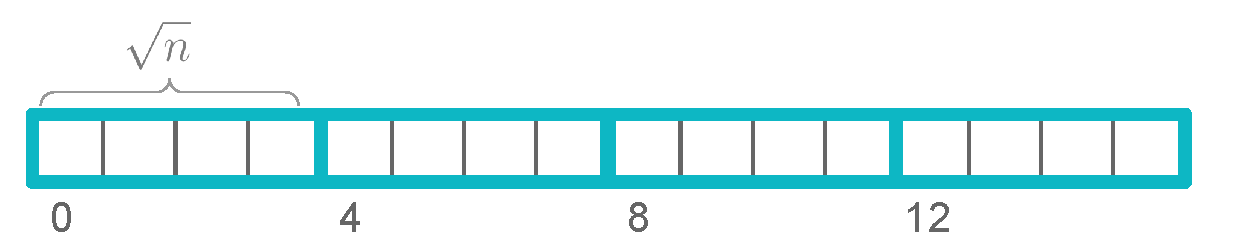
\includegraphics[scale=0.6]{chunks}\\
{\bf Figure:} The database indices are divided into $\sqrt{n}$ chunks of size $\sqrt{n}$. 
\end{center}

\paragraph{Random set.}
We will sample a random set 
of size $\sqrt{n}$ by sampling one random index from
each of the $\sqrt{n}$ chunks, as illustrated in the picture below. 


\begin{center}
    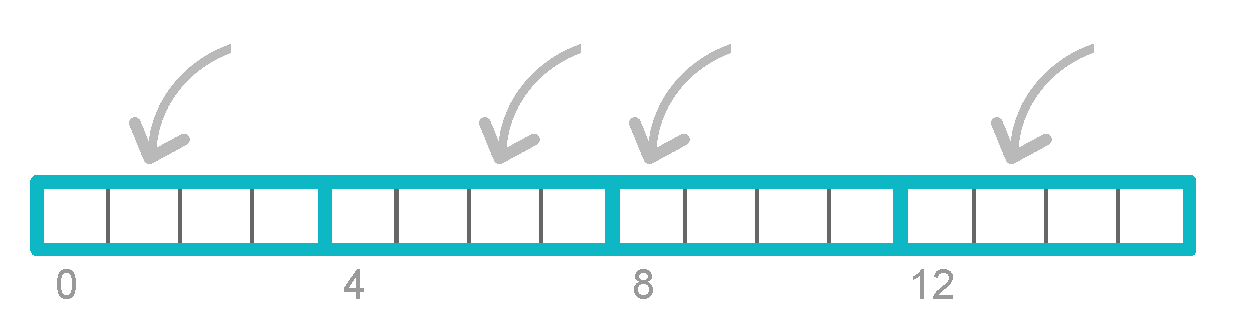
\includegraphics[scale=0.6]{piano-sample}\\
{\bf Figure:} We sample a random set of size $\sqrt{n}$ by sampling one random index per chunk.
\end{center}

Given a random set $S$ sampled according to the above procedure,
we define the notation
\[
{\sf Parity}(S) = \oplus_{i \in S}{\sf DB}[i] 
\] 


\paragraph{Describing a set with a single PRF key.}
We need a succinct way to represent each set sampled as above.
We can represent each 
set using a PRF key $\sk$.
Supposewe have a 
pseudorandom function family 
$\PRF:\{0,1\}^\lambda\times \{0,\dots,\sqrt{n}-1\}\to \{0,\dots,\sqrt{n}-1\}$. 
%associated some key $k$.
%We can use this PRF to construct a random set.
Given a PRF key $\sk \in \{0, 1\}^\lambda$, 
we can compute a pseudorandom 
index from each chunk as follows:
the index from the 
the $i$-th chunk is $\PRF_\sk(i)+i\cdot\sqrt{n}$ where $i \in \{0, \ldots, \sqrt{n}-1\}$. 
In other words,
$\PRF_\sk(i)$ outputs the offset within the 
$i$-th chunk.

%So each set only takes $\lambda$-bit to describe, 
%and the client space is $O_\lambda(\sqrt{n}\log n)$.
%

Henceforth, we use the notation ${\sf Set}(\sk)$ to denote
the pseudorandom set generated by the PRF key $\sk \in \{0, 1\}^\lambda$.
Given an index $j \in \{0,\dots,\sqrt{n}-1\}$,
we can determine if 
$j \in {\sf Set}(\sk)$ in $O_\lambda(1)$ time, 
by checking 
if $\PRF_\sk(i) + i \sqrt{n} = j$ where $i = {\sf chunk}(j)$ denotes
the chunk that index $j$ belongs to.



\paragraph{Preprocessing.}
The client wants to prepare and store the following information during the preprocessing:  
\begin{itemize}
\item 
{\bf Hint table.}
First, the client samples
$L = \widetilde{O}(\sqrt{n})$
pseudorandom sets\footnote{We use $\widetilde{O}(\cdot)$ to hide
a superlogarithmic factor.} represented by PRF keys $\sk_1, \ldots, \sk_L$.
%random sets $S_1, \ldots, S_L$.
Further, for each $i \in [L]$, the client will 
find out the parity 
$p_i = {\sf Parity}({\sf Set}(\sk_i))$, and store the parity bit alongside $\sk_i$.
The resulting table $\{(\sk_i, p_i)\}_{i \in [L]}$ 
stored by the client
is called the hint table.
Each entry $(\sk_i, p_i)$ in the hint table is called a hint.
\item 
{\bf Replacement entries.}
For each chunk $i \in \{0, \ldots, \sqrt{n}-1\}$, the client
samples $\widetilde{O}(1)$
random indices within the chunk; moreover, for each index $r$ sampled,
it wants to learn ${\sf DB}[r]$.  
As a result, the client will store $\widetilde{O}(1)$
replacement entries of the form $(r, \DB[r])$ for each chunk. 
\end{itemize}

It takes $\widetilde{O}_\lambda(\sqrt{n})$ space to
store the hint table and the replacement entries.

\begin{claim}
The client can find out all $L$ parities
as well as
the database at the sampled indices (for the replacement entries)
by making a streaming pass over the database, consuming
only $\widetilde{O}_\lambda(\sqrt{n})$ space.
\end{claim}
How to accomplish the above with a single streaming pass is left as an exercise.

\paragraph{Making a query.}
%A client makes queries in the following way. 
%Consider a client that wants to query on index $i = 6$. 
Suppose the client wants to read index
$q \in \{0, 1, \ldots, n-1\}$.
It will do the following: 
\begin{itemize}
\item 
Find a hint $(\sk^*, p^*)$
from its hint table such that $q \in {\sf Set}(\sk^*)$.
\item 
Let $i = {\sf chunk}(q)$, obtain the next unconsumed
replacement entry belonging to the $i$-th chunk, denoted $(r, \DB[r])$,
where index $r$ belongs
to the $i$-th chunk.
\item 
Let $S = {\sf Set}(\sk^*)$ but 
replace the query $q$ with $r$. 
Send $S$ to the server. 
\item 
Wait for the server to return 
$p = {\sf parity}(S)$.
Reconstruct the answer $p \oplus p^* \oplus \DB[r]$ where the client knows $\DB[r]$
from the replacement entry consumed.
\end{itemize}

Checking correctness of the answer is easy and left as an exercise.

\paragraph{Security of one query.}
Observe that the set $S$ sent to the server is indisitinguishable
from a randomly sampled set (i.e., sampling one random index per chunk).  
In particular, the client first searches for a set subject to containing the query $q$.
If the PRF were a random function, then this set would have the same distribution as
``sampling a random set subject to 
containing $q$''.
When we replace $q$ with 
%Then, it replaces $q$ with 
a random index from the same chunk, the resulting set
would have the same distribution as a randomly sampled set.

\section{Next Step: Supporting a Bounded Number of Random, Distinct Queries}
The scheme so far can support one query, but 
an issue arises if the client continues to make more queries.

The question is, 
once we make a query, 
what happens to the hint that is consumed? 
If we keep the hint, then the next time the same hint
is consumed, e.g., due to a different query, the server  
can learn the query index $q$ that was scooped out earlier.  
If we simply remove the hint, it skews the distribution of the sets 
in the hint table.
Specifically, the remaining sets have slightly lower
probability of containing the query $q$. 
This will also cause slight information leakage 
in future queries.

To avoid information leakage over multiple queries, 
the idea is the following. 
Imagine that the PRF were a random function.
Recall that the consumed set has the same distribution
as ``a randomly sampled set subject to containing the query $q$''.
When it is consumed, 
we want to replace it with a freshly sampled
set subject to containing $q$ --- of course, we will also need to know the parity
of this new set to maintain the correctness of the scheme. 

To achieve this, the client will also prepare  
some backup sets as mentioned below.

\paragraph{Backup sets.}
During preprocessing, 
for each chunk, the client will prepare 
$\widetilde{O}(1)$ number of backup sets.
A backup
set for a chunk $i \in \{0, \ldots, \sqrt{n}-1\}$ 
is sampled as follows:
sample one random index 
for every chunk $j \neq i$.
One can imagine that 
a backup set a random set except for leaving a hole in chunk $i$.
Each backup set (for some chunk $i$) 
can also be described with a PRF key $\sk$, except that 
we will never have to evaluate $\PRF_{\sk}(i)$.

\newpage
\begin{center}
    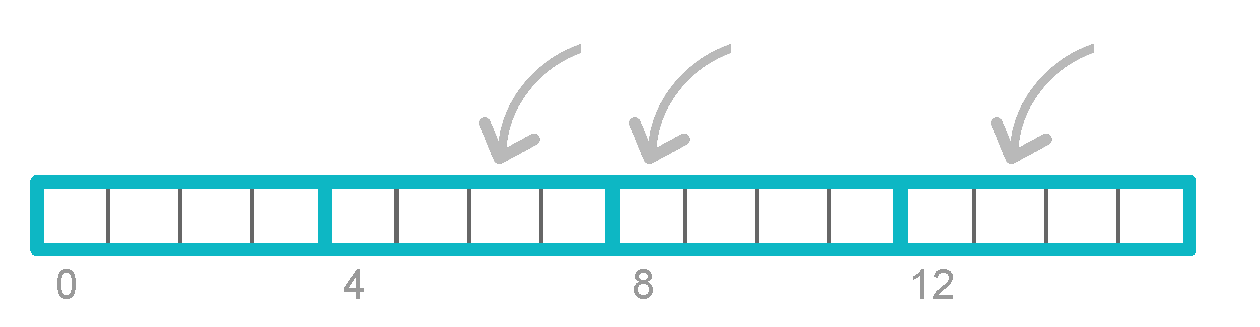
\includegraphics[scale=0.6]{piano-backupset}\\
{\bf Figure:} %The database indices are divided into $\sqrt{n}$ chunks of size $\sqrt{n}$. 
A backup set for chunk $0$ contains a random index per chunk except for chunk $0$. 
\end{center}



The client also wants to learn and store the parities of all backup sets
during preprocessing.
This can be accomplished in the same streaming pass 
mentioned above.


\paragraph{Refreshing a consumed hint.}
During a query for index $q$, 
suppose the client consumes some hint. %$(\sk^*, p^*)$. 
It will fetch
the next unconsumed backup set 
for chunk $i = {\sf chunk}(q)$.
along with its parity denoted $(\sk', p')$.
It will replace the consumed hint with $(\sk' \cup \{q\}, p' \oplus \DB[q])$,
where $\sk' \cup \{q\}$ is used to mean ``fill in the hole in the backup set represented
by $\sk'$ with $q$''; further, 
$p' \oplus \DB[q]$ is the correct parity of the set when we fill in the hole with $q$.
The client knows $\DB[q]$ because it has just reconstructed the answer to the present query.

Note that now in this scheme, 
each hint can be of the form $(\sk, p)$, or $(\sk \cup \{q\}, p)$, depending on whether
it has been refreshed or not.


\paragraph{Why bounded, random and distinct
queries.}
The scheme so far will work as long as we do not exhaust
the replacement entries and the backup sets.

Suppose there are at most $\sqrt{n}$ queries after the proprocessing,
and moreover, all queries are random and distinct.
We can think of the $\sqrt{n}$ chunks
as $\sqrt{n}$ bins, and 
each query will land in a random bin.
By Chernoff bound,  
except with negligible probability, 
no bin will receive more than super-logarithmically many queries.
This is why we provisioned $\widetilde{O}(1)$ queries (i.e., superlogarithmically many)
per chunk during preprocessing. 

\section{Supporting Unbounded and Arbitrary Queries}
 
\section{TO Edit}


\ignore{
Suppose the index we want to query is stored in some set $S_2 = (0, 6, 9, 5)$ -- note that this set can be found amongst the $\sqrt{n}$ sets with non-negligible probability. To query on this, we simply sample some random $r$ and send $S^* = (0, r, 9, 5)$ to the server. In return, we get $\mathsf{Parity}(S^*)$. With the help of our hint, we can compute $\mathsf{Parity}(S_2) \oplus \mathsf{Parity}(S^*) \oplus \mathsf{DB}[r] = \mathsf{DB}[i]$.
}




%\paragraph{Describing a pseudorandom set with a single PRF key.}

\ignore{
\begin{definition}[]
    \hfill \\
    \textbf{Parity:} Given a set of indices $S = \{i_1, i_2, \dots, i_{\sqrt{n}}\}$, we define $\mathsf{Parity}(S)$ as \hfill \\ $\mathsf{DB}(i_1) \oplus \mathsf{DB}(i_2) \oplus \dots \oplus \mathsf{DB}(i_{\sqrt{n}})$
\end{definition}
}




\ignore{In the preprocessing phase,
the client will randomly sample roughly $\Theta(\sqrt{n}\log n)$ random sets.
For each set, it samples one random index in each chunk.
The cilent will then preprocess all the  parities for those sets.
The preprocessing is done by streamingly download the whole database and dynamically update all the parities.
}


\paragraph{Compressing client hints with PRFs.}
Naively, to store all the hints, it takes $\Omega(n\log n)$ space.
Assume we have a $\PRF:\{0,1\}^\lambda\times \{0,\dots,\sqrt{n}-1\}\to \{0,\dots,\sqrt{n}-1\}$, associated some key $k$.
We can use this PRF to construct a random set.
We define the element in the $i$-th chunk to be $\PRF_k(i)+i\cdot\sqrt{n}$.
So each set only takes $\lambda$-bit to describe, and the client space is $O_\lambda(\sqrt{n}\log n)$.
%We can prove the correctness of this method with the following intuition: given some $i \in [n]$, $i$ is the index of an element within one of the $\sqrt{n}$ sets of $S$. Thus, we can get the $chunk \text{ } id$ of $i$ simply by determining which chunk it's in, and then we call the PRF on that id to get the offset, all of which is within our complexity bounds.

\paragraph{Making Queries.}
A client makes queries in the following way. Consider a client that wants to query on index $i = 6$. Suppose the index we want to query is stored in some set $S_2 = (0, 6, 9, 5)$ -- note that this set can be found amongst the $\sqrt{n}$ sets with non-negligible probability. To query on this, we simply sample some random $r$ and send $S^* = (0, r, 9, 5)$ to the server. In return, we get $\mathsf{Parity}(S^*)$. With the help of our hint, we can compute $\mathsf{Parity}(S_2) \oplus \mathsf{Parity}(S^*) \oplus \mathsf{DB}[r] = \mathsf{DB}[i]$.

However, this raises a new issue. Suppose the new index we want to query is also in $S_2$. Then if we were to send an $S^{**}$ with a different value replaced with $r$, the server would be able to recognize that $S^{**}$ is similar to $S^*$ and would then deduce some information about $i$. We also can't just delete $S_2$ to avoid this issue, because this would skew the distribution of the sets and would still give the server information about the query. The solution is that we use ``backup" sets to replace the ones we've already used.

\paragraph{Backup Sets}
Alongside the hint, each client will store a polylog number of ``backup" sets for each of the $\sqrt{n}\log n$ sets. Each backup set for chunk $j$ is stored assuming the $j$th index is missing, and the client simply stores the parity of the backup set. Examples include: $\mathsf{Parity}(0, \_\_, 9, 5)$ and $\mathsf{Parity}(0, \_\_, 8, 13)$ for the second chunk. 

\paragraph{Removing the ``Bounded" and ``Random" Queries Assumptions}
Note that within each set of $\sqrt{n}$ queries, the client can cache the results of the last $\sqrt{n}$ queries. Whenever it has a repeated query, it can make a dummy query and find the cached result. When we do the queries for the first $\sqrt{n}$ queries, we can simultaneously do the preprocessing to prepare for the next $\sqrt{n}$ queries.

\begin{center}
    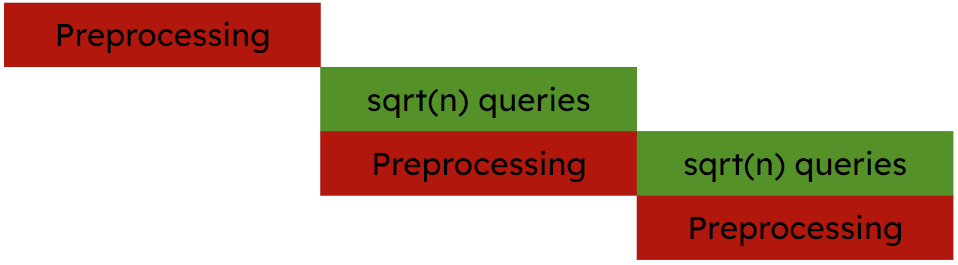
\includegraphics[scale=0.77]{scrbimg.png}
\end{center}

And as easily as that, we have removed the bounded and random queries restrictions!

\paragraph{Applications}
This scheme is much faster than non-processing PIR schemes. Because of that, it has many applications for fast secrecy. For example, \href{https://haveibeenpwned.com/}{haveibeenpwned.com}, a website that checks if a user's password has been in a data breach, would be able to more efficiently run a search on a user's password without actually ever knowing what the password is.

}
{
\newcommand{\DpfGen}{\ensuremath{{\sf DPF.Gen}}}
\newcommand{\DpfEval}{\ensuremath{{\sf DPF.Eval}}}
\newcommand{\Dpf}{\ensuremath{{\sf DPF}}}
\newcommand{\DPF}{\ensuremath{{\sf DPF}}}
\newcommand{\Prg}{\ensuremath{{\sf PRG}}}
\newcommand{\Pbc}{\ensuremath{{\sf PBC}}}

\newcommand{\GenSched}{\ensuremath{{\sf GenSchedule}}}
\newcommand{\ServerPre}{\ensuremath{{\sf ServerPreprocess}}}
\newcommand{\ClientQ}{\ensuremath{{\sf ClientQuery}}}
\newcommand{\ServerA}{\ensuremath{{\sf ServerAnswer}}}
\newcommand{\ClientD}{\ensuremath{{\sf ClientDecode}}}
\newcommand{\get}{\ensuremath{\leftarrow}}
\newcommand{\Client}{\textsf{Client}~}
\newcommand{\Server}{\textsf{Server}~}
\newcommand{\CV}{\ensuremath{{\sf CV}}}

\renewcommand{\root}{\ensuremath{{\sf root}}}

\section{Distributed Point Function and 2-server PIR with Logarithmic Communication} %~\cite{boyle2016function}}

In earlier lectures, we learned an information-theoretic 2-server PIR
scheme 
by Dvir and Gopi~\cite{dvir20162}, which
achieves $n^{O(\sqrt{\log \log n / \log n})}$ communication per query. 
%We saw that in the IT-setting, the best known upper bound on the communication of 2-server PIR scheme is by Dvir and Gopi~\cite{dvir20162}.
%The scheme achieves $n^{O(\sqrt{\log \log n / \log n})}$ communication.
In this lecture, 
we will show how to get a 2-server PIR with logarithmic communication
%from only one-way functions (OWF).
relying only on a pseudorandom 
generator (PRG). This scheme is also interesting from a practical perspective
since in practice, we can use AES to realize
the PRG, and modern CPUs have hardware acceleration
for evaluating AES. 

Recall that 
from our undergraduate cryptography course, 
we know that the existence of a PRG
is equivalent to the existence of a one-way function (OWF)~\cite{haastad1999pseudorandom}.
Also, from an earlier lecture, we learned that any 1-server
classical PIR scheme 
with non-trivial bandwidth implies
Oblivious Transfer which cannot be constructed
in a blackbox manner from OWF~\cite{IR89}. 
Therefore, the scheme we will talk about today is in the 2-server setting.

%that if we are willing to assume that one-way functions (OWF) exist, we can construct a 2-server PIR scheme with $O(\log n)$ communication.
%\mingxun{I am not sure what other sschemes you want to compare to. The IT one seems to be the most appropriate one}

\subsection{Preliminary: Pseudorandom Generator}
%This scheme use pseudorandom generators (PRG). In particular, PRG implies the existence of OWF and OWF implies the existence of PRG~\cite{haastad1999pseudorandom}. 
We will rely on a pseudorandom generator (PRG),
which takes in a short random seed and expands
the seed to a longer pseudorandom string.

\begin{definition}[PRG]
    Let $\ell(\cdot)$ be a polynomial and let 
$G:  \{0,1\}^n \rightarrow \{0,1\}^{\ell(n)}$ be a deterministic
    polynomial-time algorithm. $G$ is a \Prg \ if it has the following properties:
    \hfill
    \begin{itemize}
        \item \textbf{Expansion:} $\forall n, \ell(n) > n$.
        \item \textbf{Pseudorandomness:} for any probabilistic polynomial-time distinguisher
$D$, there exists a negligible function ${\sf negl}(\cdot)$, 
such that 
        $$\left|\Pr_{r \getr \{0, 1\}^{\ell(n)}}\left[D(r) = 1\right] - 
\Pr_{s \getr \{0, 1\}^{n}}\left[D(G(s)) = 1\right]\right| \leq {\sf negl}(n)$$ 
        %Where $r \overset{{\scriptscriptstyle\$}}{\leftarrow} \{0,1\}^{l(n)}$ and
        %$s \overset{{\scriptscriptstyle\$}}{\leftarrow} \{0,1\}^{n}$.
    \end{itemize}
\end{definition}

\subsection{Distributed Point Function}

\begin{definition}[Point function]
A point function parametrized by some point $x \in \{0, 1\}^\ell$ 
is a function that evaluates to $1$ at $x$, and evaluates to $0$ 
everywhere else.
We will henceforth use the notation $P_x \{0,1\}^{\ell} \rightarrow \{0,1\}$
to denote a point function. 
By definition, $P_x(x) = 1$ and $P_x(x') = 0$ for $x' \neq x$.
%    For $x \in\{0,1\}^*$, the point function $P_{x}:\{0,1\}^{|{x}|} \rightarrow \{0,1\}$
%    is defined by $P_{x^*}(x^*) = 1 \ and \ P_{x^*}(x) = 0$ for all $x \neq x^*$.
\end{definition}

Boyle, Gilboa and Ishai~\cite{boyle2016function} introduced the concept of a distributed point function. 
A distributed point function
is a functional secret-sharing of a point function.
In this lecture, 
we will specifically focus on a {\it 2-way} secret sharing of a point function.
Essentially, given some point function $P_{x^*}$, 
one can ``secretly share'' the function to two keys $k_L,k_R$. 
Then, for party $t \in \{L, R\}$ which
receives the key $k_t$, 
%Then, if party $t\in\{0,1\}$ receives $k_t$, 
it can evaluate the function on any point $x$ and 
get a share of the outcome denoted $\Eval(k_t, x)$. 
It is guaranteed that in every point $x$, 
$\Eval(k_L, x)\xor\Eval(k_R, x)=P_{x^*}(x)$.
In other words, it is possible to combine
the two outcome-shares to reconstruct the  
evaluation of the point function at any point. 
Finally, security of the DPF requires that  
each party $t \in \{L, R\}$ does not learn  
the ``special point'' (i.e., $x^*$) given its individual key $k_t$.


\begin{definition}[2-share \Dpf]
    A DPF is a pair of possibly randomized 
algorithms (\Gen,\Eval) with the following syntax:
    \hfill
    \begin{itemize}
        \item $\Gen(1^\lambda,x^*)$: Outputs a pair of keys $k_L,k_R$.
        \item $\Eval(1^\lambda, k,x)$: Outputs the evaluation outcome $y \in \{0,1\}$.
    \end{itemize}
    \paragraph{Correctness.} 
Correctness requires that for any $\lambda$, 
any $\ell$, 
any $x^*, x \in \{0, 1\}^{\ell}$, 
\[
\Pr\left[k_L,k_R \leftarrow \Gen(1^\lambda, x^*):\Eval(k_L,x) \oplus \Eval(k_R,x) = P_{x^*}(x)\right] = 1
\]


\paragraph{Security.} 
Security requires that 
there exists a probabilistic polynomial-time simulator $\Sim$, 
such that 
for any $\ell = \ell(\lambda)$ that is a polynomial function in $\lambda$, 
and any $x^*\in \{0,1\}^{\ell(\lambda)}$, 
the following experiments are computationally indistinguishable
for both $t  = L$ and $t = R$: 
    \begin{itemize}
        \item $\mathsf{Real}(1^\lambda, x^*)$: $k_L,k_R\get  \Gen(1^\lambda, x^*)$ and output $k_t$;
        \item $\mathsf{Ideal}(1^\lambda)$: Output $\Sim(1^\lambda, \ell)$.
    \end{itemize}
\end{definition}
Intuitively, security requires that the any individual 
key $k_L$ or $k_R$ 
can be simulated without knowledge
of the special point $x^*$.

\subsection{DPF $\Longrightarrow$ 2-Server PIR}

Given a DPF scheme henceforth denoted $(\DpfGen, \DpfEval)$, 
we can construct 
a 2-server PIR scheme as follows.
Henceforth we use $\DB \in \{0, 1\}^n$ 
to denote the database.

%Let $\DB \in \{0,1\}^{n}, i \in [n]$ and $\lambda$ be the security parameter.
%Suppose we have an efficient 2-share binary DPF scheme $\DpfGen$ and $\DpfEval$, such that the key length is $O_\lambda(\log n)$ (where $n$ is the size of the input domain), and the evaluation algorithm is efficient. 
%Then, we can have the following 2-server PIR scheme. %n the following, when the context is clear, we will omit $1^\lambda$ in the description.

\begin{enumerate}
    \item Given the query $i$, the client 
computes $(k_L,k_R) \leftarrow \DPF.\Gen(1^\lambda, i)$
    \item The client sends %$(k_L,k_R)$ to 
$k_L$ to the left server and sends $k_R$ to the right server. 
%\Server 0 and \Server 1 respectively.
    \item %For 
Each server $t \in \{L, R\}$ receives $k_t$, 
and replies 
%$t\in\{0,1\}$, \Server $t$ responds with 
$y_t := \bigoplus_{j\in [n]} \DPF.\Eval(k_t,j)\cdot \DB[j]$;
    \item the client receives
$y_L$ and $y_R$ from the two servers respectively, 
and  outputs $y_L \oplus y_R$.
\end{enumerate}

\paragraph{Correctness.} 
It is not hard to check that the answer output by the client
is correct by the DPF's correctness:  
\begin{align*} 
    y_0 \oplus y_1 & = \left(\bigoplus_{j}\DB[j]\cdot \DpfEval(k_0,j) \right) \oplus \left(\bigoplus_{j}\mathsf{DB}[j]\cdot \DPF.\Eval(k_1,j) \right) \\
    & = \left(\bigoplus_{j}\DB[j]\cdot (\DpfEval(k_0,j)\xor \DPF.\Eval(k_1,j)) \right) \\
    & = \left(\bigoplus_{j}\DB[j]\cdot P_{i}(j)\right) \\
    & = \DB[i].
\end{align*}

\paragraph{Security.}
Security of the PIR follows directly from the security of the DPF.



\subsection{DPF Construction}

\begin{figure*}[t]
    \centering

    \begin{subfigure}{0.48\textwidth}
     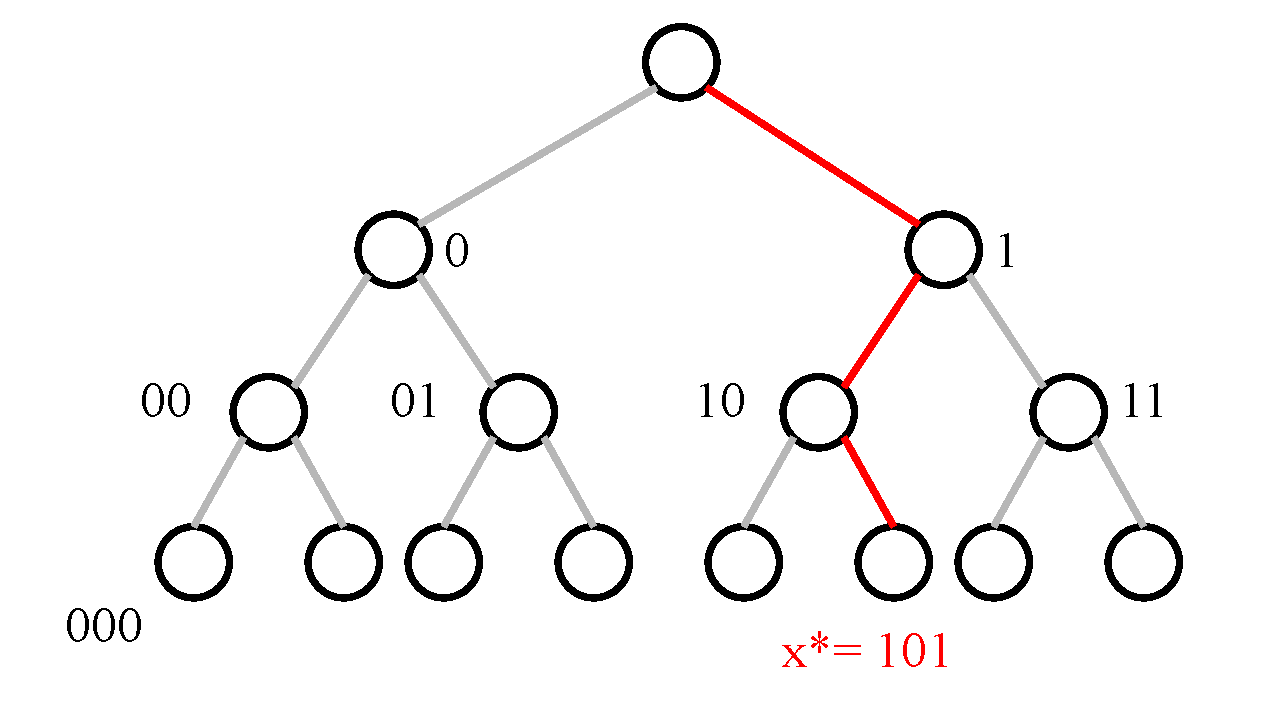
\includegraphics[width=\textwidth]{DPFtree.pdf}
     \caption{The binary tree structure used in DPF. Each node has a unique name. The path from the root to the leaf node $x^*$ is the ``special path''.}
\label{fig:tree}
    \end{subfigure}   
    \hfill
     \begin{subfigure}{0.48\textwidth}
        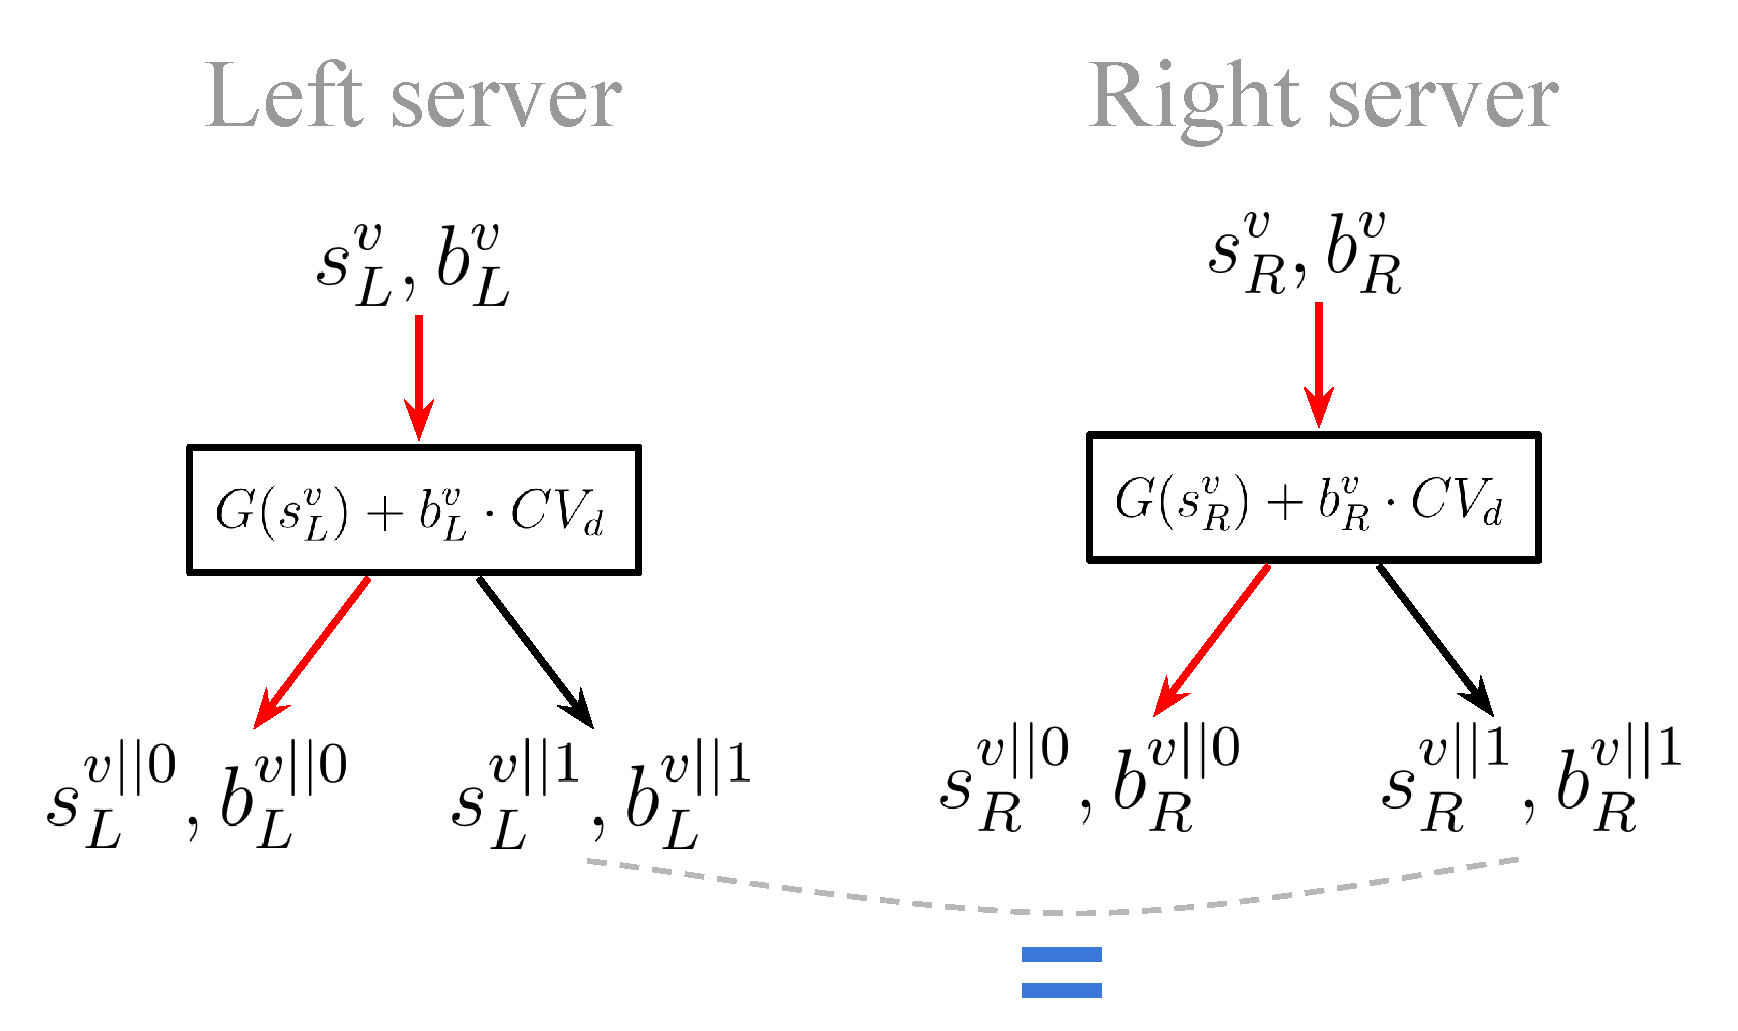
\includegraphics[width=\textwidth]{DPF1.pdf}
        \caption{Expansion during the evaluation algorithm.
The key generation computes the correction vector $\CV$ 
in a way that guarantees the following: 
for any $u$ not on the special
path, $(s_L^u, b_L^u) = (s_R^u, b_R^u)$;
and for any $u$ on the special path, 
$b_L^u \neq b_R^u$ and moreover,
the pair $(s_L^u, s_R^u)$ is indistinguishable
from two independent random strings.
%Expansion on the ``special path''. The construction enforces  the children not on the special path to have identical information, while maintaining the properties on the special path.
}
\label{fig:expand}
    \end{subfigure}
     \caption{Illustration of the DPF construction.\label{fig:dpf-demo}}
\end{figure*}





We now show how to construct an efficient DPF based on a pseudorandom
generator $G$:
 $$G: \{0,1\}^{\lambda} \rightarrow  \{0,1\}^{2\lambda + 2}. $$
The algorithm is based on a binary tree expansion idea.
%Where the series of evaluation results can be visualized as a binary tree.

\paragraph{Binary tree structure.}
Suppose we want to evaluate the DPF
at $n$ points denoted $0, 1, \ldots,  n-1$,
and we assume that $n$ is a power of $2$.

%To evaluate the DPF at all points $\{0, 1, \ldots, n-1\}$, 
Imagine that there is a binary tree
as depicted in \Cref{fig:tree}.
Each node in the tree has a name:  
the root's name is empty, and the two children of a node $v$ 
are named $v||0$ and $v||1$, respectively.
Henceforth, we say that the root is at {\it depth} $0$, the leaves
are at depth $\log n$, and so on.
Each leaf node corresponds to a point in 
$\{0, 1, \ldots, n-1\}$. In particular, it helps to express
each point in binary form.
For a point function $P_{x^*}$, 
the path from the root to the leaf node $x^*$ 
is called the special path highlighted in {\color{red}red}
in the figure. 

\paragraph{Key structure and evaluation algorithm.}
The DPF's $\Gen$ algorithm outputs two keys
$k_L = ((s_L, b_L), {\CV})$ and $k_R = ((s_R, b_R), {\CV})$,
where 
\begin{itemize}[leftmargin=7mm]
\item $s_L$ and $s_R$ are both $\lambda$-bit PRG seeds;
\item 
$b_L, b_R\in \{0, 1\}$ are flags indicating whether 
correction is necessary during the key expansion (see use
of the correction vector later in the algorithm). It
is guaranteed that $b_L \neq b_R$; 
and 
\item 
$\CV = (\CV_1, \ldots, \CV_{\log n})$ 
is a correction vector.
\end{itemize}

We will focus on the left server's perspective
for describing the evaluation algorithm. 
The right server's algorithm is the same except
that its input is $k_R$ instead of $k_L$.
Imagine that initially, the root of the tree is associated
with the pair $(s_L, b_L)$ which comes from $k_L$. 
Starting from the root, we will perform a key expansion
to compute a pair $(s_L^v, b_L^v)$
for every node $v$ in the tree.
 Each coordinate of the correction  
vector $\CV_1, \ldots, \CV_{\log n}$ 
will be consumed at each different level of the tree during the key expansion
process. 

More specifically, suppose some node $v$ has the pair
$(s_L^v, b_L^v)$, we can compute
the corresponding values at its two children $v||0$ and $v||1$ as follows
where $d$ denotes the depth of $v$'s children:
\[ 
(s_L^{v||0}, b_L^{v||0}), (s_L^{v||1}, b_L^{v||1}) \leftarrow G(s_L^v) \oplus
 \begin{cases} 
    {\bf 0} & \text{ if } b_L^v = 0; \\
    \CV_d &  \text { if } b_L^v= 1. \\
 \end{cases}
\]
Notice that the correction component $\CV_d$ is only applied if $b_L^v =1$.

At the end of the expansion process, 
for each leaf node $x$, let $b_L^x$ and $b_R^x$ be
the two bits associated with the leaf $x$ 
output by the left and right servers, respectively. 
The outcome of the DPF at point $x$ is then $b_L^x \oplus b_R^x$. 

\begin{figure*}[p]
    \begin{minipage}{\textwidth}
        \begin{mdframed}
            \begin{center}
                \textbf{Generation Algorithm:} $\Gen(1^\lambda, x^*)$
            \end{center}
            
            \paragraph{Initialization:} 
            %Repeat the following process $m$ times (indexed by $j$):
            \begin{itemize}
                \item Sample $s_L$, $s_R$ as two $\lambda$-bit random strings. 
                \item Sample a random bit $b_L$. Let $b_R=b_L\xor 1$. 
                \item Let $\{x^*[1],\dots,x^*[\log n]\}$ be $x^*$'s binary representation.
            \end{itemize}
            
            
            \paragraph{Constructing correction vectors:}  
            \begin{itemize}[label={},leftmargin=*]
                %\renewcommand\labelitemi{}
                \item Initialize $v$ to be an empty string.
                \item For $d\in \{1,\dots, \log n\}$: 
                \item 
                \begin{itemize}
                    %\item If $x^*[i]=0$, set ${\sf Keep}=L$. Otherwise, set ${\sf Keep}=R$.
                    \item Sample a random string $r\getr \{0,1\}^{\lambda}$.
                    \item Solve for 
$\CV_d\in\{0,1\}^{2\lambda+2}$ such that the following constraints
are satisfied:
                    \begin{enumerate}
                        \item[(1)] Let $(s^{v||0}_L, b^{v||0}_L), (s^{v||1}_L, b^{v||1}_L) \get G(s^v_L) \xor (b^v_L \cdot \CV_d)$; \hfill \textit{//~Expansion on the LHS}
                        \item[(2)] Let $(s^{v||0}_R, b^{v||0}_R), (s^{v||1}_R, b^{v||1}_R) \get G(s^v_R) \xor (b^v_R \cdot \CV_d)$; \hfill \textit{//~Expansion on the RHS}
                        \item[(3a)] If $x^*[d]=0$: add the following constraint: 
                        \begin{align*}
                            (s^{v||0}_L, b^{v||0}_L, s^{v||1}_L, b^{v||1}_L) \xor (s^{v||0}_R, b^{v||0}_R, s^{v||1}_R, b^{v||1}_R) = (r, 1, 0^{\lambda}, 0).
                        \end{align*}
                        \item[(3b)] If $x^*[d]=1$: add the following constraint: 
                        \begin{align*}
                            (s^{v||0}_L, b^{v||0}_L, s^{v||1}_L, b^{v||1}_L) \xor (s^{v||0}_R, b^{v||0}_R, s^{v||1}_R, b^{v||1}_R) = (0^{\lambda}, 0, r, 1).
                        \end{align*}
                        %\hfill \textit{(Force the $x^*[i]$ direction to be different and the other direction to be identical.)}
                    \end{enumerate}
%                    \item Solve the equation based on the invariant to get $\CV_d$. The equation is always solvable.
                    \item Let $v\get v||x^*[d]$.
                \end{itemize}  
            \end{itemize}
            \paragraph{Output:} Output the following $k_L, k_R$:
%that include the strings and bits on the root and the shared correction vectors:
            \begin{align*}
                k_L=(s_L, b_L, \CV_1,\dots,\CV_{\log n}) \\
                k_R=(s_R, b_R, \CV_1,\dots,\CV_{\log n})
            \end{align*}
            
        \end{mdframed}
    \end{minipage}
    \caption{The 2-way binary DPF generation algorithm.\label{fig:DPF}}
    %\caption{Detailed description of \name.\label{fig:single-server}}
\label{fig:gen}
\end{figure*}

%\begin{remark}
%Notice that if we only want to learn $\Eval(k, i)$ for a particular $i$, the computation cost will be $O(\log n)$ calls to the PRG, because we can focus on the path from the root to the $i$-th leaf and ignore other nodes.
%And on the path we only do $\log n$ expansions.
%However, if we want to evaluate $\Eval(k, i)$ for all $i\in[n]$, the computation cost will be $O(n)$ because we can simply do the evaluation on the whole tree. 
%\end{remark}



\paragraph{Key generation algorithm.}
The key generation algorithm samples  
random $s_L \getr \{0, 1\}^\lambda$ and $s_R \getr \{0, 1\}^\lambda$ 
at the root nodes for the left and right servers, respectively.
It chooses a random bit $b_L \getr\{0, 1\}$ 
and sets $b_R = b_L \oplus 1$.
Then, it will choose the correction vector $\CV_1, \ldots, \CV_{\log n}$
in a way such that 
the following {\bf invariants} are guaranteed for each
tree node $v$:

\begin{itemize}[leftmargin=7mm]
\item 
For every tree node $v$
that is not on the special path leading to $x^*$, 
it must be that $(s_L^v, b_L^v) = (s_R^v, b_R^v)$.
\item 
For every tree node $v$
that is on the special path leading to $x^*$, 
it must be that $b_L^v \neq b_R^v$,
and moreover, the pair $(s_L^v, s_R^v)$ 
is indistinguishable from two independent $\lambda$-bit random 
strings.
\end{itemize}

Note that for some node $v$, if 
$(s_L^v, b_L^v) = (s_R^v, b_R^v)$
is already guaranteed, then 
for any node $u$ that is in the 
subtree of $v$,  
$(s_L^u, b_L^u) = (s_R^u, b_R^u)$
is automatically guaranteed because
the left and right servers
will behave identically when the apply the same 
expansion algorithm to compute 
all values in the subtree of $v$.
Therefore, in the key generation algorithm, 
we can compute the correction vector $\CV$
using only the special path, to maintain
the aforementioned invariants. 

The detailed key generation algorithm is specified
in \Cref{fig:gen}.


%\paragraph{The key structure.} The $\Gen$ algorithm outputs two keys, $k_L, k_R$. For each key $k_t$ where $t\in\{0,1\}$, it contains the ``root'' information as a $\lambda$-bit random string $s$ and a bit $b\in\{0,1\}$. It also contains $\log n$ ``correction vectors'' $\CV_1, \dots, \CV_{\log n}$, each of size $2\lambda+2$ bit. $k_L, k_R$ will share the same sets of correction vectors. 
%We will see how they are constructed later. 



\ignore{
\paragraph{Evaluation algorithm.} 
Given a key containing $s,b$ and $\CV_1,\dots,\CV_{\log n}$, the evaluation algorithm is as follows.
We consider a binary tree with $\log n + 1$ levels and $n$ leaves (assume $n$ is a power of 2). 
The root is on the $0$-th level and the leaves are on the $\log n$-th level.
For the $2^i$ nodes on the $i$-th level, we use $i$-bit to label them: the labels are from $\underbrace{0,\dots,0}_{i~\text{bits}}$ to $\underbrace{1,\dots,1}_{i~\text{bits}}$.
The root is labeled with an empty string.
See Figure~\ref{fig:dpf-demo} for the demonstration.
Now given the string $s^v$ and the bit $b^v$ on a node $v\in \{0,1\}^{i-1}$ on the level $i-1$, the strings and the bits on the nodes $v||0$ and $v||1$ are:
\[ 
s^{v||0} || b^{v||0} || s^{v||1} || b^{v||1} \leftarrow G(s^v) \oplus
 \begin{cases} 
    0 & b^v = 0; \\
    \CV_d & b^v= 1. \\
 \end{cases}
\]
That is, $s^{v||0}, b^{v||0}$ are the string and bit on its left child, and $s^{v||1}, b^{v||1}$ are the string and bit on its right child.
We first use the PRG to expand $s^v$, then if $b^v=1$, we will apply the correction vector to the evaluation results. 
Finally, given the evaluation point $i\in[n]$, the bit on the $i$-th leaf will be $\Eval(k, i)$.

Notice that if we only want to learn $\Eval(k, i)$ for a particular $i$, the computation cost will be $O(\log n)$ calls to the PRG, because we can focus on the path from the root to the $i$-th leaf and ignore other nodes.
%And on the path we only do $\log n$ expansions.
However, if we want to evaluate $\Eval(k, i)$ for all $i\in[n]$, the computation cost will be $O(n)$ because we can simply do the evaluation on the whole tree. 
}




\ignore{
\paragraph{Generation Algorithm.} The generation algorithm needs to generate two correlated keys, such that when we look at the bit at the $x$-th leaves on the left server and the right server, (say $b^{x}_{L}$ and $b^{x}_{R}$), it must that $b^{x}_{L}\xor b^{x}_{R}=P_{x^*}(x)$. In fact, we want to ensure the following stronger properties.
Say on a particular node $v$, we denote the information evaluated by the left server and the right server as $(s^v_L,b^v_L)$ and $(s^v_R,b^v_R)$, respectively.
We also denote the path from the root to the $x^*$-th leaf as the ``special path''.

\begin{enumerate}
    \item If the node $v$ is on the special path (i.e., $v$ is a prefix of the binary representation of $x^*$), then $b^v_L\ne b^v_R$, and $s^v_L$ and $s^v_R$ are independent.
    
    \item Otherwise, $(s^v_L,b^v_L)=(s^v_R,b^v_R)$.
\end{enumerate}

The properties also hold for the leaf nodes, which is sufficient to prove the correctness of the DPF. 
We now see the how to ensure these properties.
We have the first lemma, which can be proved by a simple induction argument.
}

\ignore{
\begin{lemma}
    If on some particular node $v$, $(s^v_L,b^v_L)=(s^v_R,b^v_R)$, then the information on the subtrees of $v$ will be identical, regardless of $\CV_1,\dots,\CV_{\log n}$. That is, for every $v'$ that has prefix $v$, $(s^{v'}_L,b^{v'}_L)=(s^{v'}_R,b^{v'}_R)$. 
\end{lemma}

This lemma shows that we only need to focus on the ``special path''. We can sample the roots first by sampling two random strings $s_L,s_R$ and let $b_L$ and $b_R$ be two different bits. 
Then, we can just ``simulate'' the expansion process on the special path, and then set up the correction vector according to the target properties. 
Given a node $v$ on the special path ($v$ is a prefix of $x^*$), say $v$ is on the $i-1$ level.
Now assuming the correction vector $\CV_i$ is a \textit{variable} to be determined.
We can still following the evaluation algorithm, but all the expansion results, $s^{v||0}_L, b^{v||0}_L, s^{v||1}_L, b^{v||1}_L$, $s^{v||0}_R, b^{v||0}_R, s^{v||1}_R, b^{v||1}_R$, will be temporally some linear expressions of the variable $\CV_i$.
Then, we can enforce the invariants.
Say $v||0$ is still the prefix of $x$ (the other case is symmetric). We require that 
\begin{itemize}
    \item \textit{Invariant on the special path.} 1) The xor-sum of $s^{v||0}_L$ and $s^{v||0}_R$ is a freshly sample random string $r$ (ensuring they are independent); 2) $b^{v||0}_L$ and $b^{v||0}_L$ are different.
    \item \textit{Invariant on other nodes.} $(s^{v||1}_L,b^{v||1}_L)=(s^{v||1}_R,b^{v||1}_R)$.
\end{itemize}
Now these invariants set up a simple linear equation and we can easily solve the value of $\CV_i$.
The equation is always solvable because $b^v_L$ and $b^v_R$ are different.
Thus, the $\CV_i$ will always and only affect the expansion on the one side.
Note that the second invariant just enforces that the whole subtree of $v||1$ will be identical, and we just need to go to the child $v||0$ and derive $\CV_{i+1}$ based on $s^{v||0}_L, b^{v||0}_L$ and $s^{v||0}_R, b^{v||0}_R$.
We run this algorithm from level $1$ to level $\log n$ and get $\CV_1,\dots,\CV_{\log n}$.
The algorithm is presented in Figure~\ref{fig:DPF} and an example is presented in Figure~\ref{fig:dpf-demo}.
}

\paragraph{Analysis.}
The correctness can be verified by 
inductively checking that the aforementioned invariants hold
at every level.  
%doing an induction proof from level $1$ to level $\log n$.
The security analysis is referred to~\cite{boyle2016function}. 
\elaine{prove security?}
It is not hard to see that 
the key size is $\lambda+1+\log n\cdot (2\lambda+2)=O_\lambda(\log n)$.



 \section{Batch-PIR}

 \subsection{Motivation}
    So far, every PIR scheme we have seen only retrieves 1 bit at a time. 
    In many use cases, the client may want to fetch up to $Q$ database entries at the same time. 
    The navie solution is just to repeat the single-query algorithm $Q$ times.
    For instance, to compute Q queries using a single-query PIR scheme with $O(n)$ computation, it requires $O(Qn)$ computation.
    Batch-PIR aims to handle multiple parallel queries at the same time, reducing the
     amortized cost.
     
     
\subsection{A simple load-balancing scheme}

Given an $n$ bit long database and $Q=o(n)$ queries, we load-balance the database into $\frac{Q}{\log Q}$ buckets -- we use a hash function to hash each database entry to a bucket (by hashing their index).
Then, given the $Q$ queries, we again use the hash function to place the queries to the buckets. 
In expectation, each bucket will have $\log Q$ queries. 
Based on the balls-into-bins argument, each bucket will have no more than $\lambda \log Q$ queries with $1-\negl(\lambda)$ probability.
Therefore, we just do $\lambda \log Q$ PIR queries in each bucket (possibly dummy queries) to retrieve the target entries. 
This ensures the success probability is at least $1-\negl(\lambda)$.

\paragraph{Security.}
We are always making fix number of queries ($\lambda \log Q$ PIR queries in each bucket), so the scheme is secure by a reduction to the security of the underlying PIR scheme.

\paragraph{Cost.}
Moreover, say the underlying single-query PIR computation cost is linear in the size of the database.
We are making $\lambda \log Q$ queries to each bucket, and the total size of the buckets is just $n$. 
Therefore, the total computation cost is $O(\lambda \log Q n)$. 
So if $Q>\lambda \log Q$, this simple scheme saves computation.


     
     
\subsection{Cuckoo Hashing based scheme~\cite{angel2018pir}}

Angel et al.~\cite{angel2018pir} proposed SealPIR that uses cuckoo hashing to do batch PIR.
    
    \paragraph{Cuckoo Hashing}
    \begin{definition}[Cuckoo hashing]
        Given $n$ balls, $b$ buckets, and $w$
independent hash functions $h_0$, $\cdots$ , $h_{w}$ that map a ball to a
random bucket, compute $w$ candidate buckets for each ball by
applying the $w$ hash functions. For each ball $x$, place $x$ in any
empty candidate bucket. If none of the $w$ candidate buckets
are empty, select one at random, remove the ball currently in
that bucket ($x_{\text{old}}$), place $x$ in the bucket, and re-insert $x_{\text{old}}$. If
re-inserting $x_{\text{old}}$ causes another ball to be removed, this process
continues recursively until we finish the insertion or a maximum number of iterations is achieved.
    \end{definition} \
    
\paragraph{Batch PIR based on Cuckoo Hashing.}   
The scheme is as follows.
\begin{itemize}
    \item \textbf{Serer encoding.} Given an $n$ bit database, $b$ buckets, and $w$ hash functions, we hash each entry in the database (using their index as the key) to all $w$ candidate buckets and store it there.
    This results in a encoded database that each original entry is replicated $w$ times.
    The server will share the hash functions to the client.
    
    \item \textbf{Client scheduling.} Given the $Q$ queries, the client use the cuckoo hashing method to insert (or say, schedule) the queries to the buckets (again, using the indices as the keys).
    Our target is that each bucket has at most one query, and all query can be inserted in one of its candidate bucket.
    
    \item \textbf{Client query.}. Now the client just makes one query in each bucket. If the client successfully insert all queries earlier, it can then proceed to learn all the target entries because the server has inserted the entries in all the candidate buckets.
\end{itemize}

An example can be found in Figure~\ref{fig:sealpir}.
   
The authors used 3 hash functions for encoding and set the number of buckets $b = 1.5Q$. For $Q\geq 200$, the author showed that the chance of failure during
the scheduling phase is $\leq 2^{-40}$.
Notice that this is not cryptographically neligible. 
To enforce negligible failure probability, we can introduce a size $\lambda$ stash of the cuckoo hash table.
That is, the stash stores at most $\lambda$ elements that fail to be inserted. 
Then, the client also has to make additional $\lambda$ PIR queries to the whole database.
This ensures the failure probability to be $\negl(\lambda)$.

\paragraph{Cost Analysis.} 
Assume the underlying single-query PIR scheme is linear.
The client will make one query in each bucket and the total bucket size is $wn$.
Also, the client needs to make $\lambda$ additional query to the whole database to ensure negligible failure probability.
Then, the computation cost for the $Q$ queries are just $(w+\lambda)n$.

    
    
\begin{figure*}
    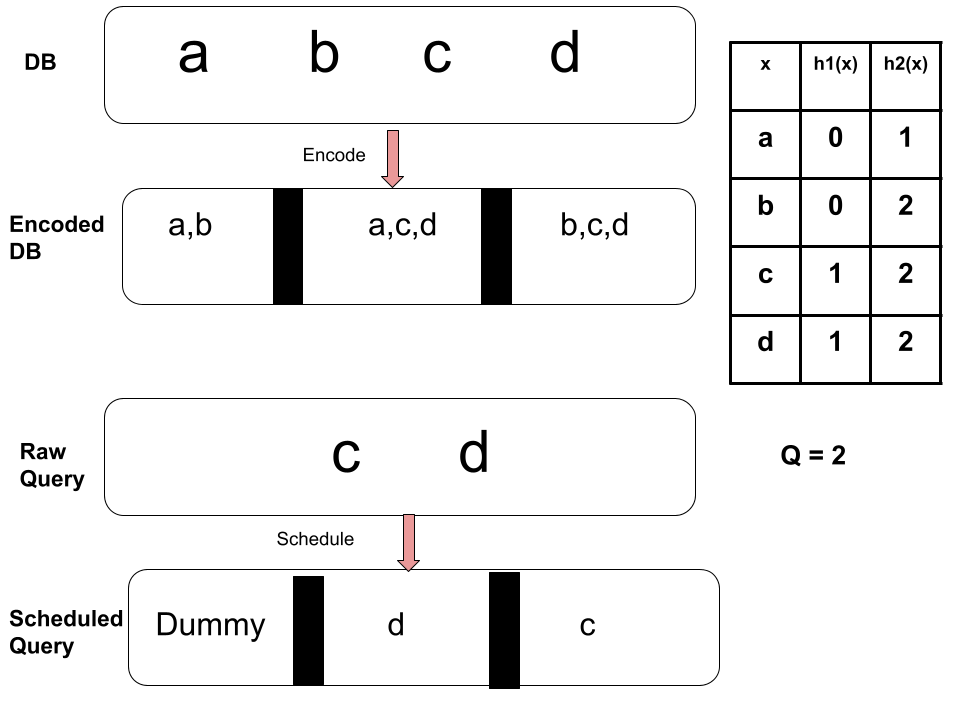
\includegraphics[scale=0.45]{scribimg_batchpir.png}
    \caption{An example of the cuckoo hashing based batch PIR. \label{fig:sealpir}}
\end{figure*}












\ignore{

%%%%%%%%%%%%%

Intuitively, this just applies all hash functions to an entry. If all buckets it gets hashed to are
taken, it will choose a random bucket, remove the ball currently in there and re-insert
using the same procedure. \\
\paragraph{Probabilistic Batch Codes}
\begin{definition}[Batch Code ~\cite{angel2018pir}]
    A (n, m, k, b)-batch code B takes as input a collection DB of n
    elements, and produces a set of m codewords, C, distributed
    among b buckets. Formally, $B : DB \rightarrow (C_0,..., C_{b})$, where
    $|Ci|$ is the number of codewords in bucket i, and the sum of
    codewords across all buckets is $m = \sum_{i=0}^{b-1}|Ci| \geq n$.
    The goal of these codes is two-fold. First, they ensure that any k elements
    from DB can be retrieved from the b buckets by fetching at most
    one codeword from each bucket. Second, they keep the number
    of total codewords, m, lower than $k \cdot n$.
\end{definition}
Batch codes incur a large network overhead by guaranteeing completeness in that it
is always possible to retrive k codewords by querying k distinct buckets. By adding possibility of failure p,
bandwidth can be shaved off at the cost of a chance of query failure. Applying this relaxation
results in a Probabilistic Batch Code, which is how SealPIR is able to encode a database
into multiple sub-databases that can be queried simultaneously with PIR. Informally, they are defined by 3 functions:
\begin{itemize}
    \item \textbf{\sf Encode(DB):} Split the database and replicate entries accordingly.
    \item \textbf{\sf GenSchedule(W):} Generate a query to each subdatabase such that all desired items are retrieved.
    \item \textbf{\sf Decode(I):} Extracts individual responses from the server response.
\end{itemize}
A formal definition and construction using reverse hashing can be found on page 6 of ~\cite{angel2018pir}


\subsection{The SealPIR scheme}

\paragraph{Intuition} The main idea is to build a \Pbc \ over the PIR database. The only major modifications
are to GenSchedule and Decode, where the equeries must be modified to be PIR queries. While failures in the query scheduling phase are
possible, the authors tune the parameters to make the likelihood very low.
\\
\paragraph{Notation}
Let \Pbc = $(\mathsf{Encode},\GenSched,\mathsf{Decode})$ be a Probabilistic Batch code constructed using Cuckoo hashing. Additionally,
Let PIR = (\ServerPre,\ClientQ,\ServerA,\ClientD) be a PIR scheme.

\paragraph{\sf SealPIRPreprocess} Given w independent hash functions $H = (h_1,...,h_w)$ and \DB, output b buckets $B = {B_1,...,B_b}$, where:
$$\sf B_i = SealPIRPreprocess(s_i),(s_0,...s_b) = encode(DB) $$
\paragraph{\sf SealPIRQuery} For a set of Q queries $q_1,...,q_b$, and Cuckoo hashing algorithm CK:
\begin{enumerate}
    \item Client computes $\sigma \leftarrow GenSchedule(Q)$
    \item if $\sigma \neq \perp$ goto (3) else  return failure
    \item Client computes $(q_1,...q_b) \leftarrow (ClientQuery(B_0,\sigma[0]),...,ClientQuery(B_Q,\sigma[b]))$ and sends the result to the server
\end{enumerate}
Where $\sigma \in \{\{1,....,b\}\}^b$ maps queries to the bucket the query should go to. $\sigma == \perp$ if there were two indices mapped to the same bucket.

\paragraph{\sf SealPIRAnswer} Server computes and sends $$r_i = \ServerA(B_i,\sigma[i]), \forall i \in [Q]$$ back to client.
\paragraph{\sf SealPIRDecode} To retreive the answer to the ith query, the client computes:
$$a_i \leftarrow \sf Decode(ClientDecode(r_i))$$

%%%%%%%%%%%%%



}

}
{
%\usepackage{xspace}

\newcommand{\bits}{\{0,1\}}
\newcommand{\bfu}{\mathbf{u}}
\newcommand{\bfv}{\mathbf{v}}
\newcommand{\bfp}{\mathbf{p}}
\newcommand{\bfz}{\mathbf{z}}
\newcommand{\bfx}{\mathbf{x}}
\newcommand{\bfy}{\mathbf{y}}

\newcommand{\calR}{\mathcal{R}}

\newcommand{\CNextMsg}{\ensuremath{{\sf C Next Msg}}}
\newcommand{\SNextMsg}{\ensuremath{{\sf S Next Msg}}}
\newcommand{\CNext}{\ensuremath{{\sf C Next}}}
\newcommand{\SNext}{\ensuremath{{\sf S Next}}}
\newcommand{\Cstp}{\ensuremath{{\sf Cst'}}}
\newcommand{\Cst}{\ensuremath{{\sf Cst}}}
\newcommand{\msg}{\ensuremath{{\sf msg}}}
\newcommand{\msgp}{\ensuremath{{\sf msg'}}}
\newcommand{\Coutput}{\ensuremath{{\sf Reconstr}}}
\newcommand{\ans}{\ensuremath{{\sf ans}}}
\newcommand{\Ccoins}{\ensuremath{{\sf Ccoins}}}
\newcommand{\Scoins}{\ensuremath{{\sf Scoins}}}
%\newcommand{\Comm}{\ensuremath{{\sf Comm}}}
\newcommand{\Expt}{\ensuremath{{\sf Expt}}}
\newcommand{\coin}{\ensuremath{{\sf coin}}}
\newcommand{\View}{\ensuremath{{\sf View}}}
%\newcommand{\negl}{\ensuremath{{\sf negl}}}
\newcommand{\PPT}{PPT }
\newcommand{\Out}{\ensuremath{{\sf Out}}}
\newcommand{\OWF}{\ensuremath{{\sf OWF}}}
\newcommand{\OT}{\ensuremath{{\sf OT}}}
\newcommand{\PIR}{\ensuremath{{\sf PIR}}}
\newcommand{\Server}{\ensuremath{{\sf Server}}}
\newcommand{\Client}{\ensuremath{{\sf Client}}}
\newcommand{\Alice}{\ensuremath{{\sf Alice}}}
\newcommand{\Bob}{\ensuremath{{\sf Bob}}}
%\newcommand{\getr}{\ensuremath{~{\overset{\$}{\leftarrow}}}~}
\newcommand{\get}{\ensuremath{\leftarrow}}
\newcommand{\E}{\ensuremath{{\bf E}}}
\newcommand{\out}{\ensuremath{{\sf out}}}
%\newcommand{\PRF}{\ensuremath{{\sf PRF}}}
\newcommand{\prob}{\ensuremath{\mathbb{P}}}
\newcommand{\known}{\ensuremath{{\sf known}}}
\newcommand{\enc}{\ensuremath{{\sf enc}}}
\newcommand{\db}{\ensuremath{{\sf DB}}}
\newcommand{\bbad}{\ensuremath{{\sf b_{bad}}}}
\newcommand{\bgood}{\ensuremath{{\sf b_{good}}}}

\setlength{\parindent}{0pt}
%This is our final lecture on private information retrieval. 
In this lecture, we will prove a lower bound about the client space and server computation 
tradeoff for preprocessing PIR schemes. 
%For the proof, we will use techniques from complexity theory literature.
We will borrow techniques for proving time-space tradeoff
from the complexity theory literature.

Specifically, we consider a 1-server preprocessing PIR scheme 
in which 
the client and the server 
first performs some preprocessing over the database $\DB\in \{0, 1\}^n$.
The preprocessing can perform  
an unbounded amount 
of computation, at the end of which 
the client obtains an $S$-bit hint
at the end of the preprocessing, and the server stores only the original database
itself, and no extra information. 
Then, the client engages in a query protocol with the server,
to learn the database at some index  
$i \in [n]$.
To answer the query, the server is allowed to read at most $T$ locations of the database. 
For such a preprocessing PIR scheme, we will prove a tradeoff
between $S$ and $T$ as stated in the following theorem: 

\begin{theorem}[Time space tradeoff for preprocessing PIR~\cite{CK20}]
    Given a 1-server preprocessing PIR, 
        let $S$ be the client space, and let $T$ be the server compuation per query. 
    Then,  
    $(S+1)(T+1) \ge N$. \elaine{TODO: edit the theorem based on what we can prove later}
\label{thm:lb}
\end{theorem}

\paragraph{Piano.}
Recall that in an earlier lecture, 
we covered Piano~\cite{piano}, a preprocessing 1-server PIR scheme. 
It uses the client-specific preprocessing model, meaning that each client has a subscription phase with the server, during which it will perform preprocessing. Piano enjoys 
the following performance bounds:
\begin{itemize}[leftmargin=7mm]
    \item Client space: $\widetilde{O}(\sqrt{n})$
where $\widetilde{O}(\cdot)$ hides a(n  arbitrarily small) superlogarithmic function.
    \item Communication per query: $O(\sqrt{n})$
    \item Server computation per query: ${O}(\sqrt{n})$
\end{itemize}

We can see that Piano achieves optimal 
client space and server computation tradeoff (up to polylogarithmic factors)
in light of \Cref{thm:lb}.
%Consider the server computation and client space trade-off. For PIANO, this trade-off [Client Space: $\widetilde{O}(\sqrt{n})$, Compute per Query: $\widetilde{O}(\sqrt{n})$] is nearly optimal up to poly-log factors. 


%This is because of the following lower bound.
%\paragraph{Space/Computation Lower Bound}


%This lower bound holds even for a scheme that supports 1 query, regardless of server space, bandwidth, and amount of preprocessing work. 

Before proving \Cref{thm:lb}, 
we first prove a time-space tradeoff for a classical problem
called the Yao's box problem~\cite{yao}, and we shall
see why 
Yao's box problem is closely related to preprocessing PIR.

\section{Yao's Box Problem}
We have a server with $N$ boxes, each covering a bit. Note that this is not a PIR scheme, because it does not provide any privacy guarantees.

\paragraph{Preprocessing Phase}
Client and server can open all bits, and run arbitrary and unbounded computations. However, we have a constraint that at the end of the preprocessing, client can only store $S$ bits of information.

\paragraph{Query}
Client wants to know the i-th bit. We allow the client and server to have unbounded communication and work. We have a constraint that the server can open at most $T$ boxes and it cannot open box $i$.

\paragraph{Upper Bound}
\begin{enumerate}
    \item Divide the $N$ boxes into $\sqrt{N}$ segments. 
    \item Preprocessing Phase: Have the client store the parity of each segment.
    \item Query Phase ($i$): Server opens every box in $i$'s segment except $i$ and sends the parity back to the client. As the client knows the parity of each segment, it can easily reconstruct the value of bit $i$.
\end{enumerate}
Here, $S = \sqrt{N}$ and $T = \sqrt{N} - 1$

\paragraph{Lower Bound} \label{box_lower}
\begin{theorem}
    $S(T+1) \ge N$ 
\end{theorem}
\begin{proof}
    We will be using an encoding type argument. Consider the following experiment.
    \begin{enumerate}
        \item Run preprocessing
        \item Define an empty set called $\known = \{\}$. In each step $i$, the client finds the smallest $q_i \notin \known$, queries $q_i$.

        With this step, $\known \impliedby \known \cup \{q_i\} \cup {\text{all boxes opened during query}}$
        \item If $\known \neq [N]$, break. Otherwise, repeat step 2 again.
    \end{enumerate}

    Let the ``client's hint" denote whatever information that the client stores after the preprocessing phase. The hint is at most $S$ bits long.
    
    Define the encoding $\enc$ for this process as follows: 
    \[\enc = \text{client's hint} + \text{all ``newly opened" boxes in all queries}\]

    We write ``newly opened" because we do not want to include values that have already been recorded in the encoding.
    \vspace{5mm}
    
    By Shannon's theorem, we will show that $|\enc| \ge N$.

    Let $t_1, t_2, ...\ t_k$ be the number of newly opened boxes at each step $i \in [k]$. 
    
    Note here that we have the power of \textbf{plus one}; if I open $t$ boxes, I end up learning $t+1$ new bits. This is because I also learn the value of the query without opening its box.

    Thus, the $\known$ set increments with the following pattern.

    \begin{itemize}
        \item We newly open $t_1$ boxes: $\known$ increments by $t_1 + 1$
        \item We newly open $t_2$ boxes: $\known$ increments by $t_2 + 1$
        \item and so on...
    \end{itemize}

    Thus, we have that $\sum_{i = 1}^k (t_i + 1)\ge N$. Let $t = \frac{\sum_{i = 1}^k t_i}{k}$. Note that $t$ is the average number of boxes opened on each iteration so it must be upper bounded by $T$, the maximum number of boxes that can be opened in an iteration. Since we repeat the steps until $\known = [N]$, we have that
    \[\sum_{i = 1}^k (t_i + 1)\ge N \implies (t+1)k \ge N \implies k\ge \frac{N}{t+1} \tag{1}\]

    The encoding size is $S + \sum_{i=1}^k t_k = S + tk$. By Shannon's we have that $S + tk \ge N$. By (1), we have that 
    \begin{align*}
        S + tk &\ge N \\
        &\implies S + t \frac{N}{t+1} \ge N \tag{By (1)}\\
        &\implies S(t+1) \ge N \tag{Simplification}\\
        &\implies S(T+1) \ge N \tag{As $t \le T$}
    \end{align*}
\end{proof}

\section{PIR Lower Bound}
Using our knowledge of Yao's Box Problem, let's know try to prove the PIR lower bound.
\begin{theorem}
    Suppose we have a 1 server prepossessing PIR with perfect correctness and $negl(n)$ privacy loss with client space $S$ and server computation $T$ per query. Then,
    \[(S+1)(T+1) \ge  N \ \ \cite{CK20}\]
\end{theorem}
This lower bound holds even for computationally private schemes. It holds even for a single query, regardless of bandwidth, server space, even when preprocessing can be unbounded. However, we have a restriction that the server stores the original database and nothing else. That is, it does not store any encoding of the database.

\vspace{5mm}

For the proof, we will show that a solution to the PIR problem can be used to construct an algorithm to solve a probabilistic version of Yao's Box Problem.

\paragraph{Probabilistic Yao's Box Problem}
Suppose we have a working PIR scheme. Now, we will construct a solution to probabilistic Yao's Box Problem as follows:

\begin{itemize}
    \item Client's Hint: PIR's hint
    \item Query for $i \in [N]$: Run PIR for query $i$. If server looks at $\db[i]$, then output ``error".
\end{itemize}

% We stop at 46:00 in the recording.
We want to show the following. Given that PIRExpt: $i \xleftarrow{\$} [N]$, PIR preprocessing, PIR query on $i$,
\[p =\prob[\text{PIRExpt opens $i$}] \le \frac{T}{N} + \negl(N)\]

That is, we want to show that if we run a PIR query with the a random index $i$, the probability we open that index is small.

For a fixed $i$, define the following probability $p_i = \prob[\text{PIR on $i$ looks at $i$}].$ Then, 
\[p =\frac{1}{N} \sum_i p^i\]

Assume for the sake of contradiction that  $p > \frac{T}{N} + \mu$, where $\mu$ is non-negligible.

Let $p_{ji} = \prob[\text{PIR on $j$ opens $i$}]$. Since our scheme is private, the different indices should be computationally indistinguishable. Thus, this probability should be equally distributed. As a result,
\[p_{ji} = \prob[\text{PIR on $j$ opens $i$}] \ge p_i - \negl(N)\]

\begin{align*}
    E[\text{server work for PIR on $j$}] &\ge \sum_{i=1}^N p_{ji} \\
    &\ge \sum_{i=1}^N (p_{i} - \negl(N))\\
    &= Np - \negl(N) \tag{By def. of $p$}\\
    &> T + \mu N - \negl(N) \tag{As $p > \frac{T}{N} + \mu$}\\ 
\end{align*}

Thus, we have a contradiction because the expected number of locations the server needs to look at is strictly greater than $T$. Thus, we have shown that 

\[\prob[\text{PIRExpt opens $i$}] \le \frac{T}{N} + \negl(N)\]

\vspace{5mm}

Shifting our focus back to Yao's Box problem with probabilistic correctness on random index, the probabilistic correctness is
\[\prob[i \xleftarrow{\$} \text{correct for $i$}] \ge 1 - \frac{T}{N} - \negl(N)\]

\paragraph{Encoding Argument}
Randomness comes from two parts: the preprocessing part (the client's hint), and the query part. With this in mind, we will be using an augmented version of the encoding type argument in \ref{box_lower}.

Consider the following experiment.
\begin{enumerate}
    \item Run preprocessing, and choose a ``reasonably good hint." Initially, let the encoding be just the hint. We will add to this encoding as we go forward.
    \item Define an empty set called $\known = \{\}$
    \item In each step $i$, find the smallest $q_i \notin \known$. 
    \begin{itemize}
        \item If $\exists$ online coins such that query $q_i$ will give the correct answer, choose the lexicographically smallest coin. Execute query.
        \[\known \impliedby \cup \{q_i\} \cup \{\text{all newly opened}\}\]
        Add ``newly opened" to encoding.
        \item Else add $q_i$-th bit to the encoding.
    \end{itemize}
    \item Repeat until $\known = [N]$.
    
\end{enumerate}

A hint is bad for $i \in [N]$ if $\prob[\text{query $i$ correct} | \text{hint}] = 0$. That is, there does not exist an online coin such that the query is correct.

\begin{claim}
    $\exists$ hint that's bad for at most $T + 1$ location.
\end{claim}
\begin{proof}
    If all hints are bad for  more than $T+1$ locations, then
    \[\prob[i \in [N], \text{correct on $i$}] < 1 - \frac{T+1}{N}\]

    We have a contradiction, because it disagrees with our probabilistic correctness result above.
\end{proof}

Finally, we can reason about the encoding length. 

Suppose the worst case where the hint is bad for exactly $T+1$ locations. Let $\bbad$ be the encoding of the ``newly opened" boxes in the bad queries, and $\bgood$ be the encoding of the ``newly opened boxes in the good queries.
\begin{itemize}
    \item $|\bbad| = T + 1$, as each bad iteration adds one bit, and we have $T+1$ iterations.
    \item To find $|\bgood|$, we repeat the argument from \ref{box_lower}. Let $t_1, t_2, ...\ t_k$ be the number of newly opened boxes at each good step $i \in [k]$.

    By the ``plus one" argument, we have that $\sum_{i = 1}^k (t_i + 1)\ge N - (T + 1)$. We subtract $T + 1$ here because those indices have been handled by the bad iterations.
    
    Let $t = \frac{\sum_{i = 1}^k t_i}{k}$. Then as before, we have $k\ge \frac{N}{t+1}$
    \begin{align*}
        \sum_{i = 1}^k (t_i + 1)&\ge N - (T + 1) \\
        &\implies tk + k \ge N - T - 1 \\
        &\implies k \ge \frac{N - T - 1}{t+1}
    \end{align*}

    Thus, $|\bgood| = tk \ge t\frac{N - T - 1}{t+1}$
\end{itemize}

With the information above, we can mek the following conclusion.
\begin{align*}
    |\enc| &= S + |\bgood| + |\bbad| \ge N \\
    &\implies S + t\frac{N - T - 1}{t+1} + T + 1 \ge N \\
    &\implies S(t+1) + T + 1 \ge N \tag{By simplification}\\
    &\implies (S+1)(T+1) \ge N \tag{As $t$ upper bounded by $T$}
\end{align*}

\qed

}




\bibliographystyle{alpha}
\bibliography{refs.bib}
\end{document}
